\newpage
\section*{Appendix: Extra Experiments}
\label{sec:appendix}

%\subsection{Case Study for Feature Extraction}


\subsection*{Exp-5: Case Study for User Clustering}

In this section, we show the results of our system \sys{} for User Clustering. We carefully analyzed the statistical information of four groups obtained from user clustering.

\stab(1) Most users of group one are male (as shown in Sub-Fig. \ref{fig:subfig1:fig11}), and Sub-Fig. \ref{fig:subfig1:fig12} shows that they are mainly in Beijing(����). The amount of their followees is mostly similar as their followers (as shown in Sub-Fig. \ref{fig:subfig1:fig14}). The most active time of this group is mainly between 10 am and 12 am (as shown in Sub-Fig. \ref{fig:subfig1:fig15} and \ref{fig:subfig1:fig16}).

\stab(2) Mostly users of group two are  female (as shown in Sub-Fig. \ref{fig:subfig2:fig21}) and are also mainly in Beijing (����) (shown as Sub-Fig. \ref{fig:subfig2:fig22}). Similar to group one, most of them have followees close to followers (as shown in Sub-Fig. \ref{fig:subfig2:fig24}). The most active time of this group is mainly between 10 pm and 12 pm (as shown in Sub-Fig. \ref{fig:subfig2:fig25} and \ref{fig:subfig2:fig26}).

\stab(3) Most users of group three are male (as shown in Sub-Fig. \ref{fig:subfig3:fig31}). They come from a wide range of provinces (as shown in Sub-Fig. \ref{fig:subfig3:fig32}). Most of them have number of followers far more than followees (as shown in Sub-Fig. \ref{fig:subfig3:fig34}). The most active time of this group is mainly in 10-12 am and 10-12 pm (as shown in Sub-Fig. \ref{fig:subfig3:fig35} and \ref{fig:subfig3:fig36}).

\stab(4) Most users of group four are female (as shown in Sub-Fig. \ref{fig:subfig4:fig41}), and they come from a wide range of provinces just as group three (as shown in Sub-Fig. \ref{fig:subfig4:fig42}). Most of these users have the amount  of followers far more than followees (as shown in Sub-Fig. \ref{fig:subfig4:fig44}). And the most active time of these users is mainly between 10 pm and 12 pm (as shown in Sub-Fig. \ref{fig:subfig4:fig45} and \ref{fig:subfig4:fig46}).

According to Sub-Figs. \ref{fig:subfig1:fig13}, \ref{fig:subfig2:fig23}, \ref{fig:subfig3:fig33} and \ref{fig:subfig4:fig43},
the number distribution of microblogs for four groups is similar with each other.
We visualize each group's long-term interest expressed as words cloud (shown in Sub-Figs. \ref{fig:subfig1:fig19}, \ref{fig:subfig2:fig29}, \ref{fig:subfig3:fig39} and \ref{fig:subfig4:fig49}). As we can see, group one and group three have similar interests.

\begin{figure*}
  \centering
  \subfigure{
  \label{fig:subfig1:fig11}
      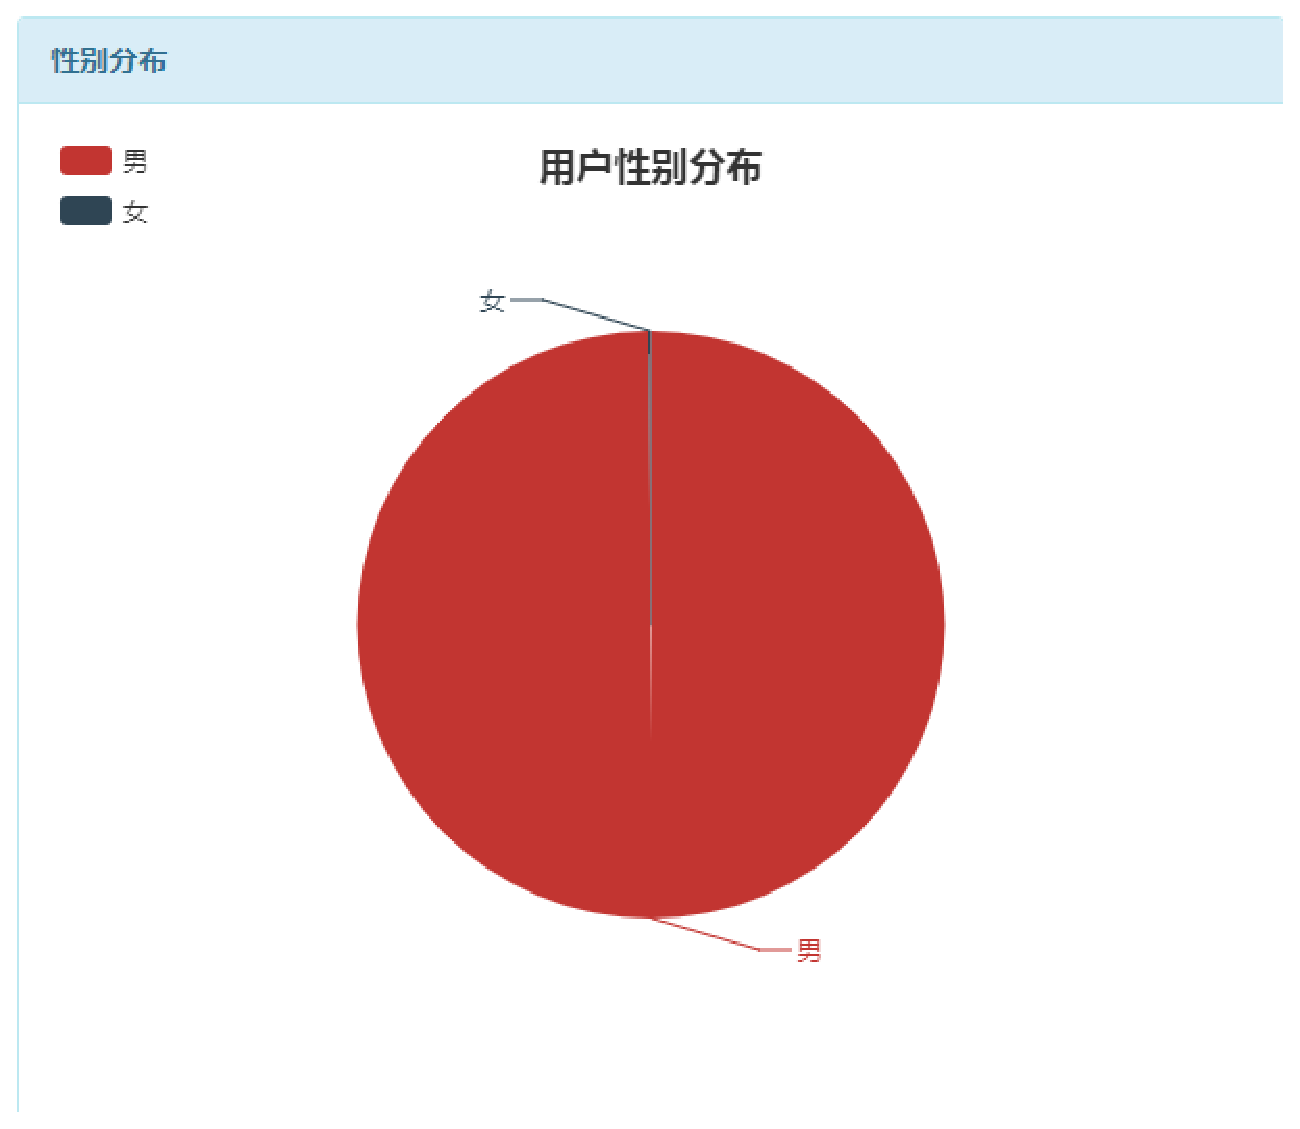
\includegraphics[width=0.23\textwidth]{IMAGE/group-images/11.eps}}
  \subfigure{
  \label{fig:subfig1:fig12}
      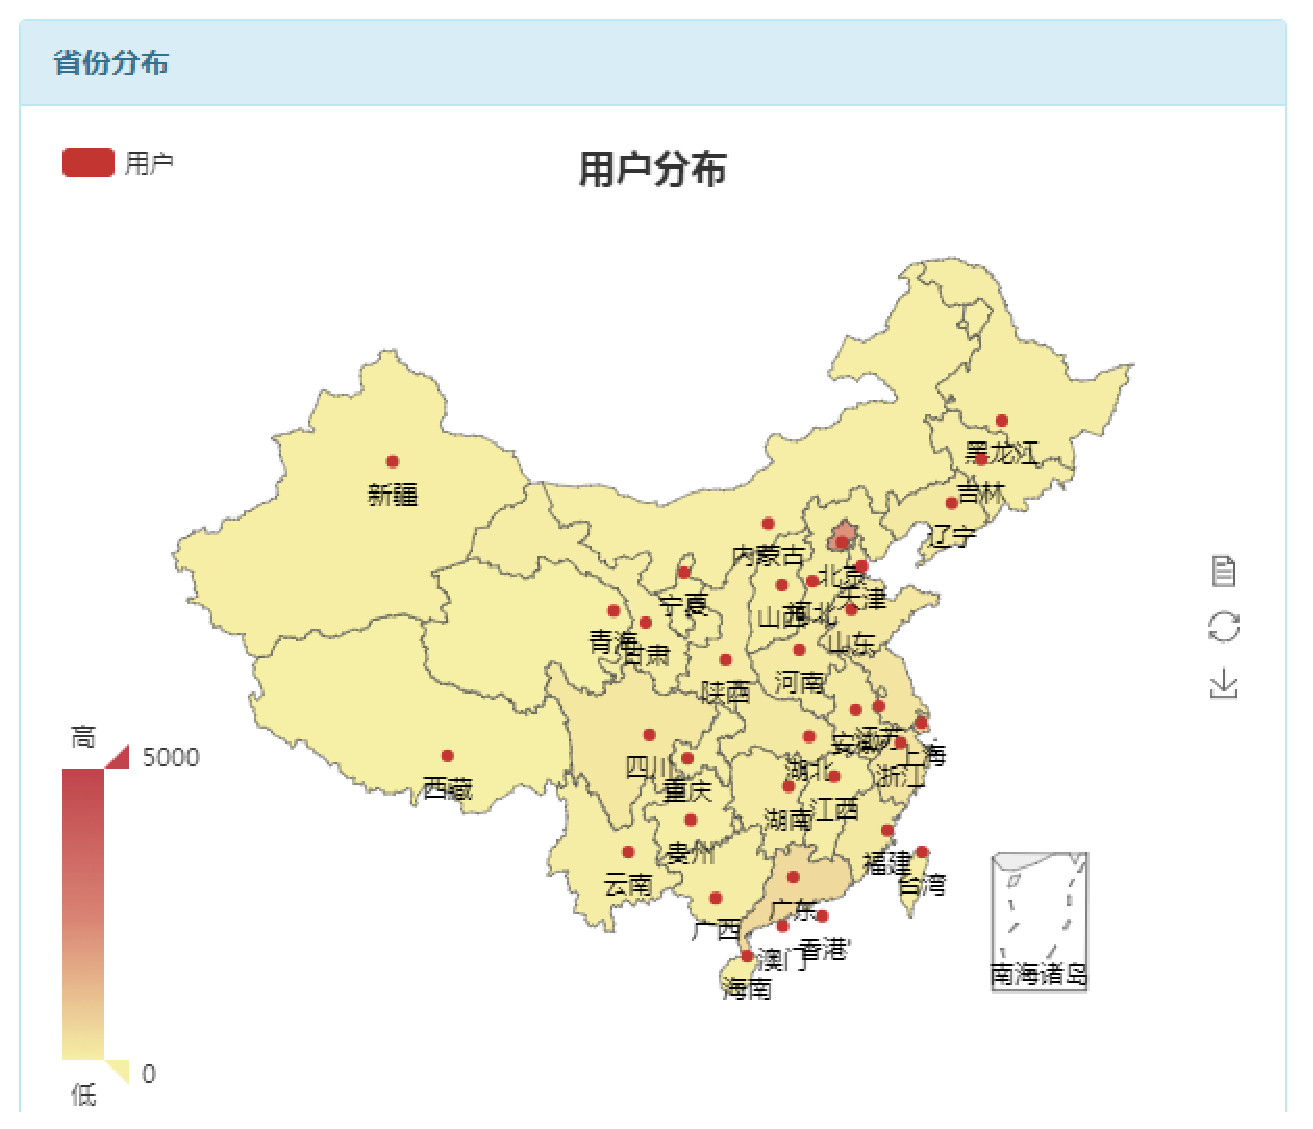
\includegraphics[width=0.23\textwidth]{IMAGE/group-images/12.eps}}
  \subfigure{
  \label{fig:subfig1:fig13}
      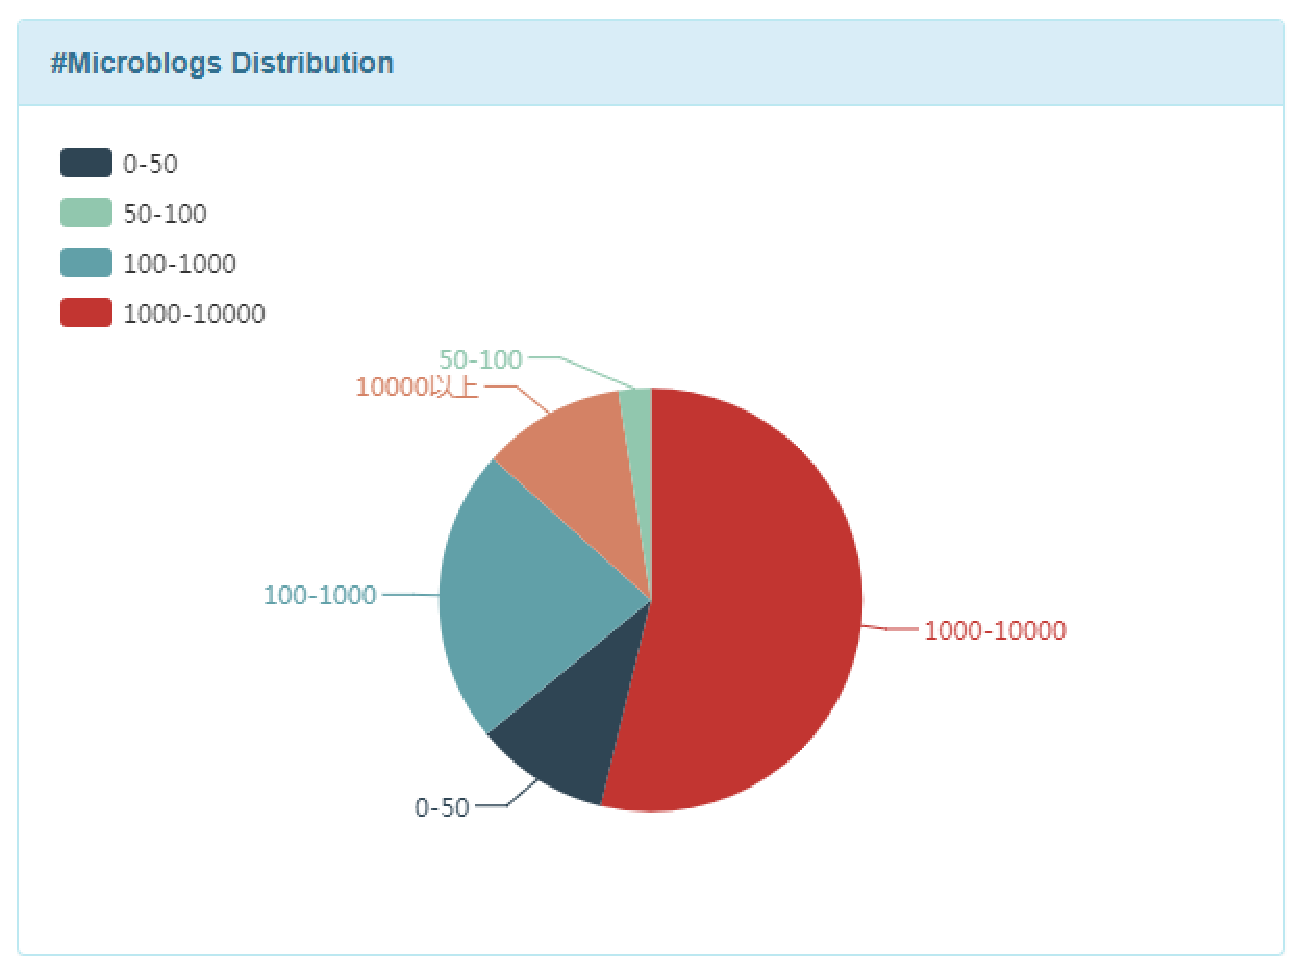
\includegraphics[width=0.23\textwidth]{IMAGE/group-images/13.eps}}
  \subfigure{
  \label{fig:subfig1:fig14}
      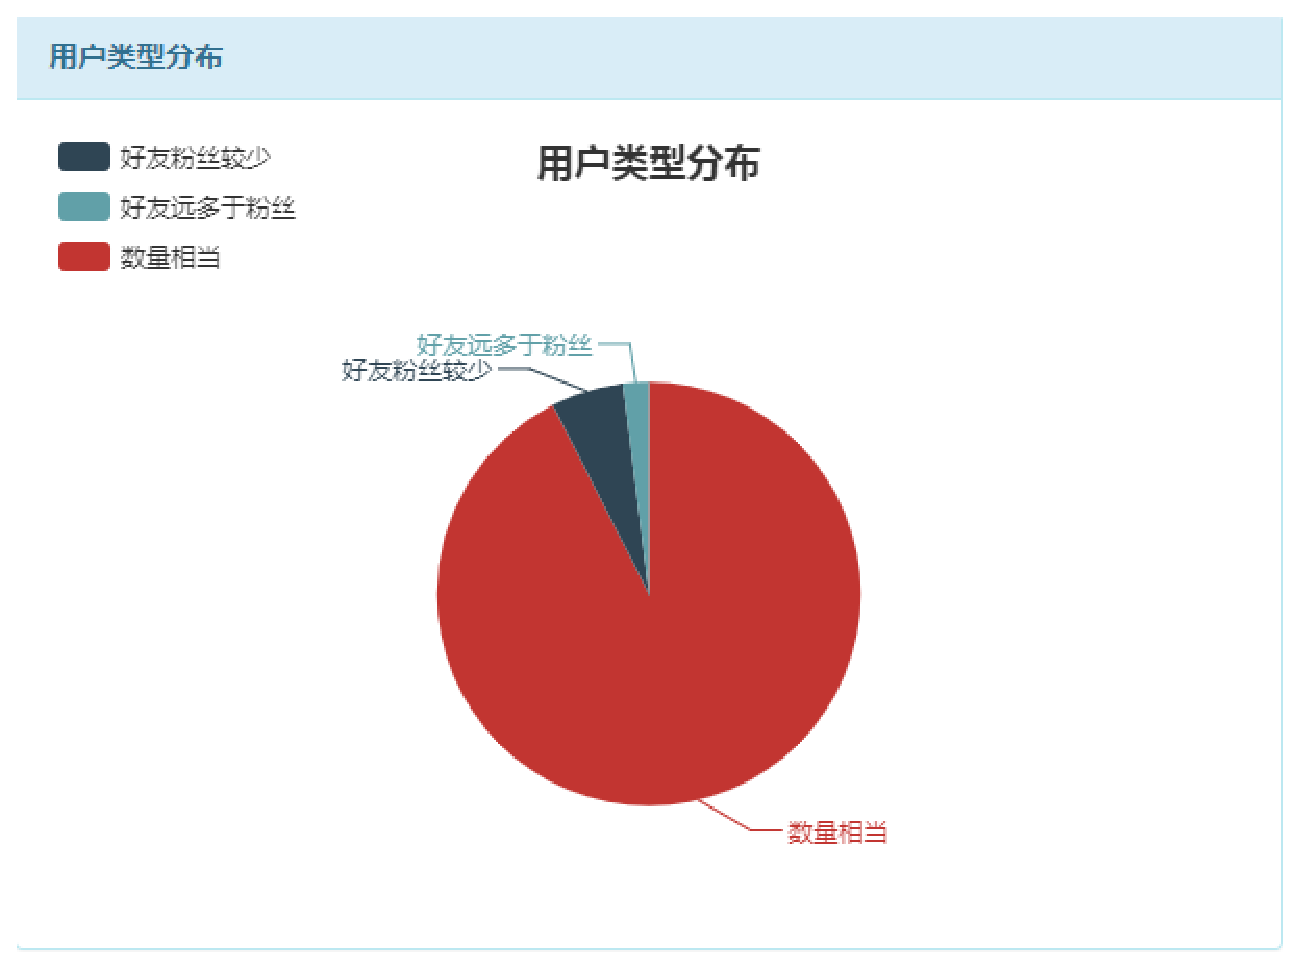
\includegraphics[width=0.23\textwidth]{IMAGE/group-images/14.eps}}
  \subfigure{
  \label{fig:subfig1:fig15}
      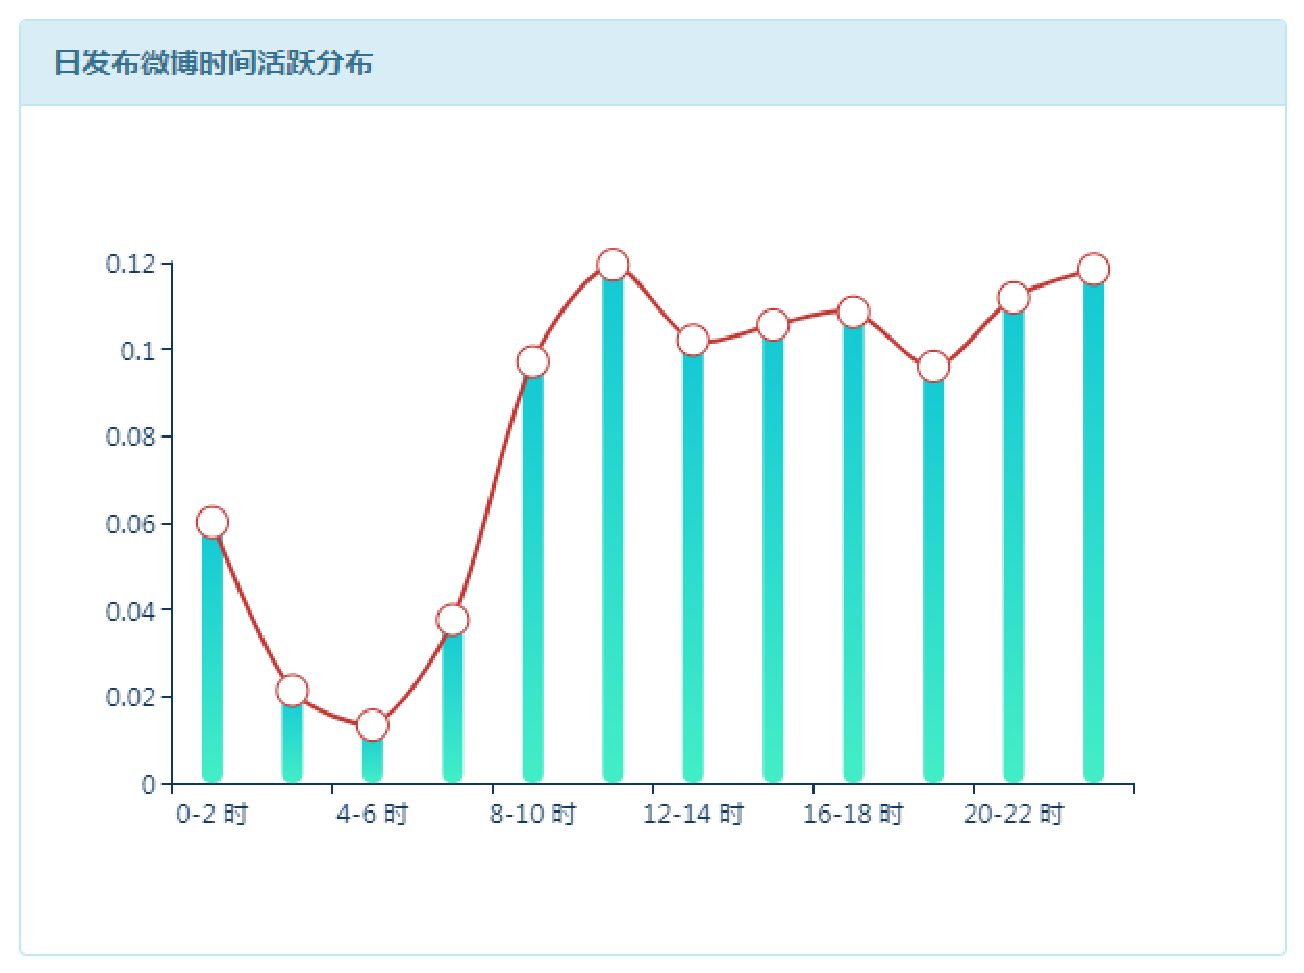
\includegraphics[width=0.23\textwidth]{IMAGE/group-images/15.eps}}
  \subfigure{
  \label{fig:subfig1:fig16}
      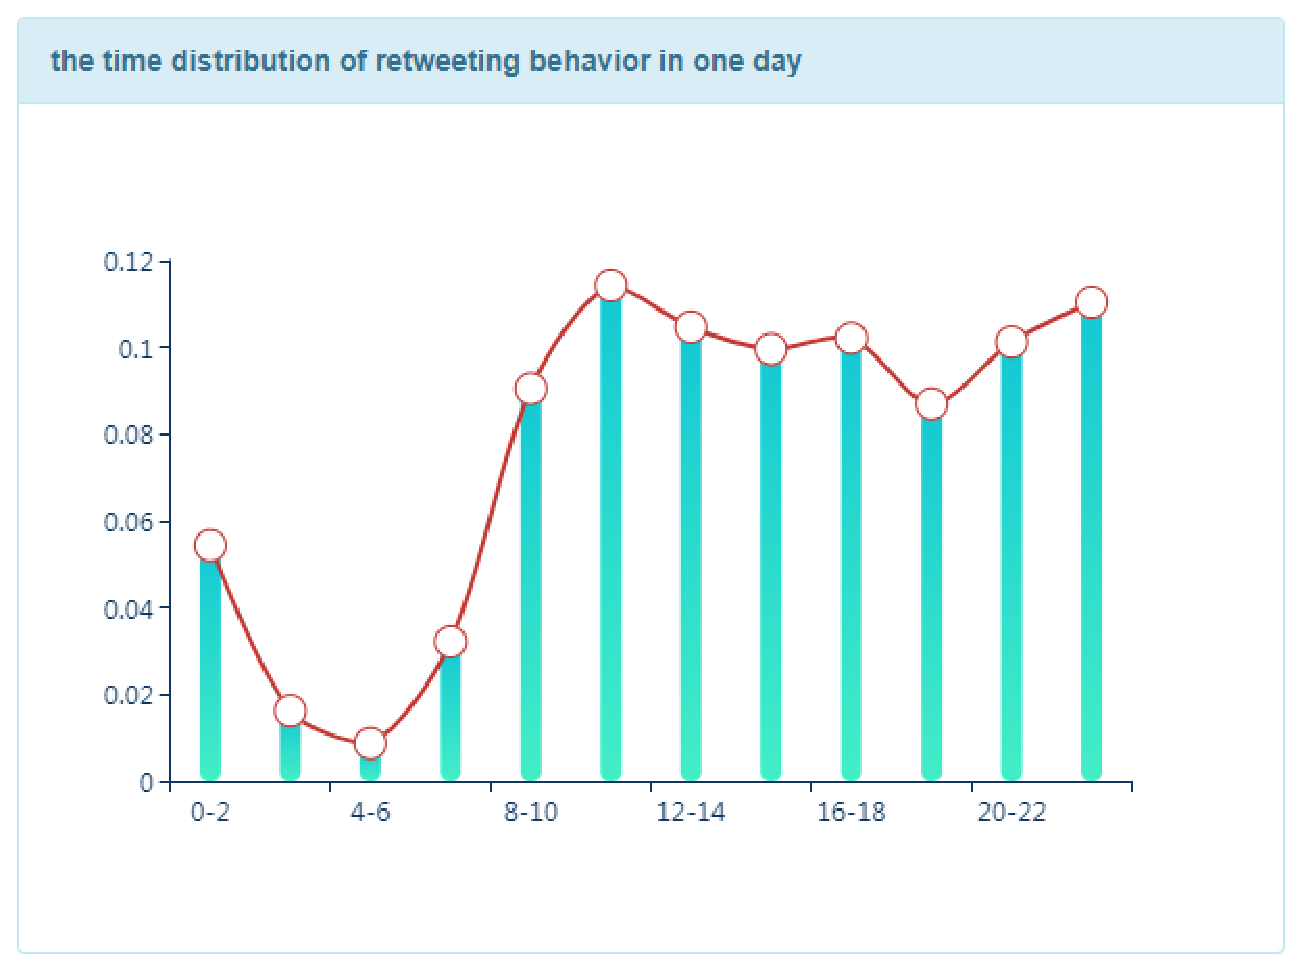
\includegraphics[width=0.23\textwidth]{IMAGE/group-images/16.eps}}
  \subfigure{
  \label{fig:subfig1:fig17}
      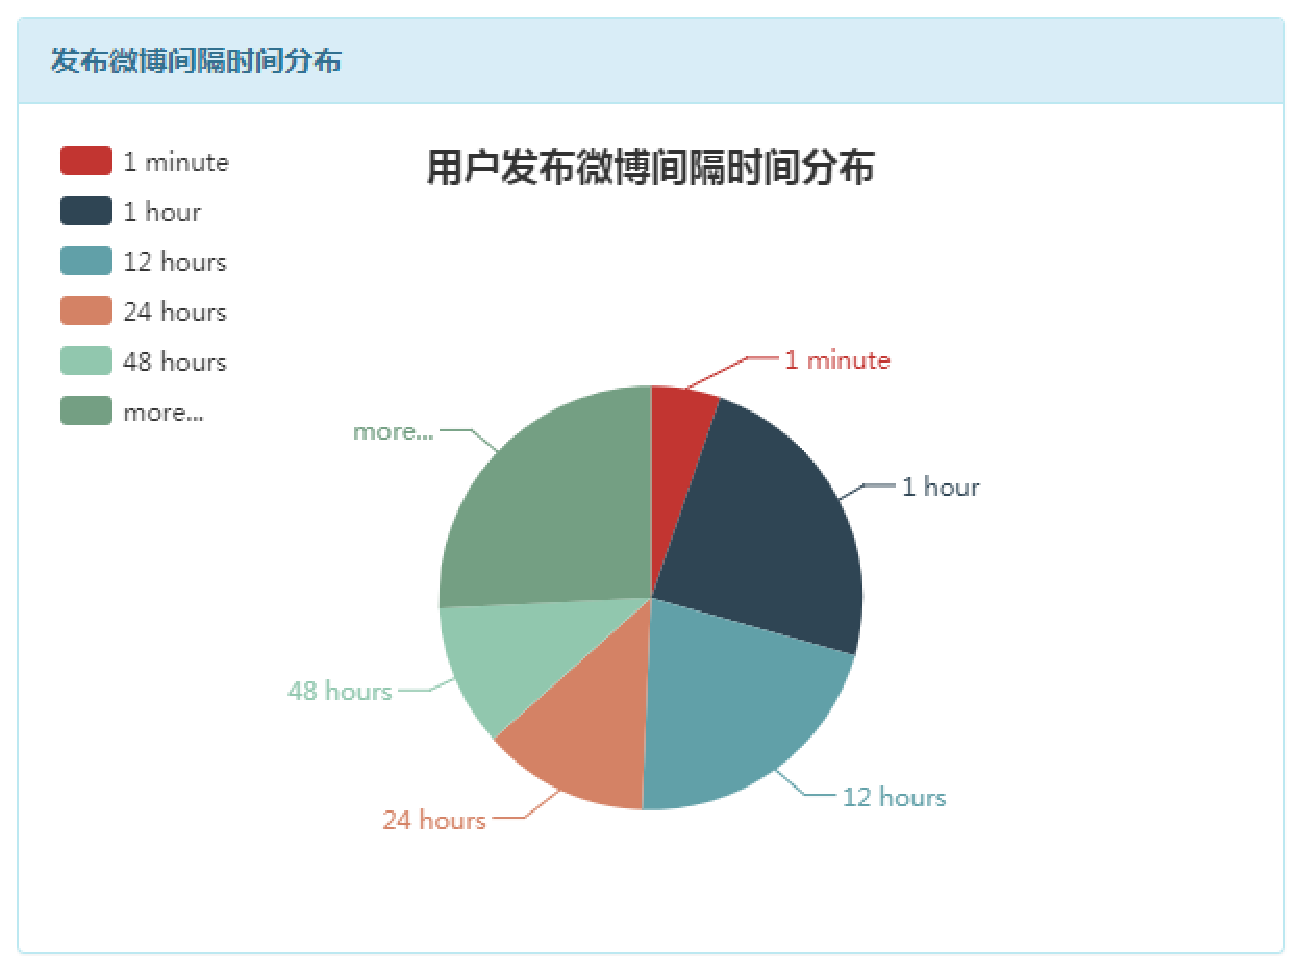
\includegraphics[width=0.23\textwidth]{IMAGE/group-images/17.eps}}
  \subfigure{
  \label{fig:subfig1:fig18}
      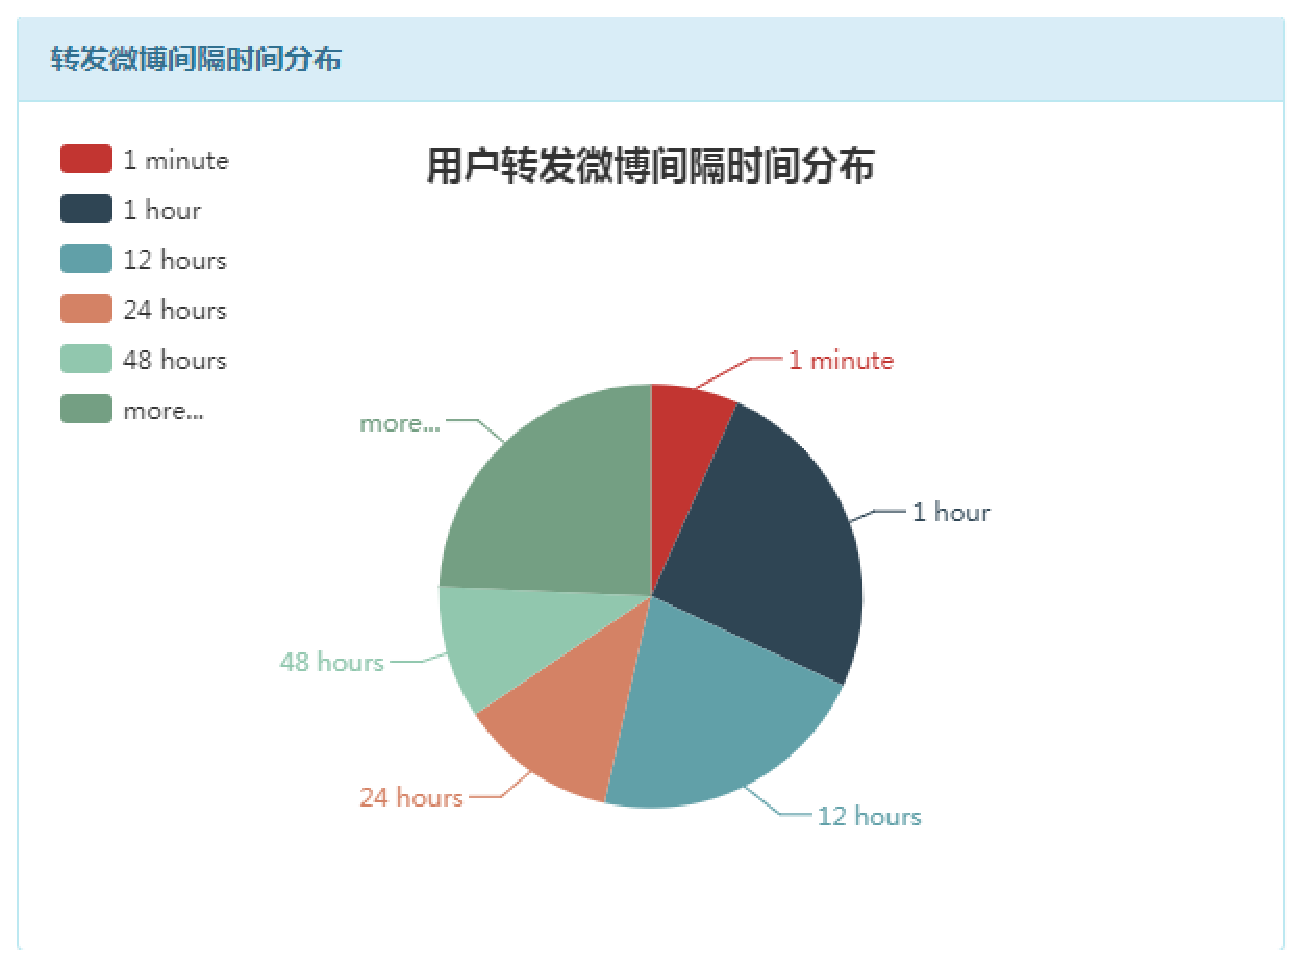
\includegraphics[width=0.23\textwidth]{IMAGE/group-images/18.eps}}
  \subfigure{
  \label{fig:subfig1:fig19}
      
\includegraphics[width=0.23\textwidth]{IMAGE/group-images/19.eps}}
  \caption{The Statistics of User Group One}
  \label{fig:subfig1} %% label for entire figure
\end{figure*}

\begin{figure*}
  \centering
  \subfigure{
  \label{fig:subfig2:fig21}
      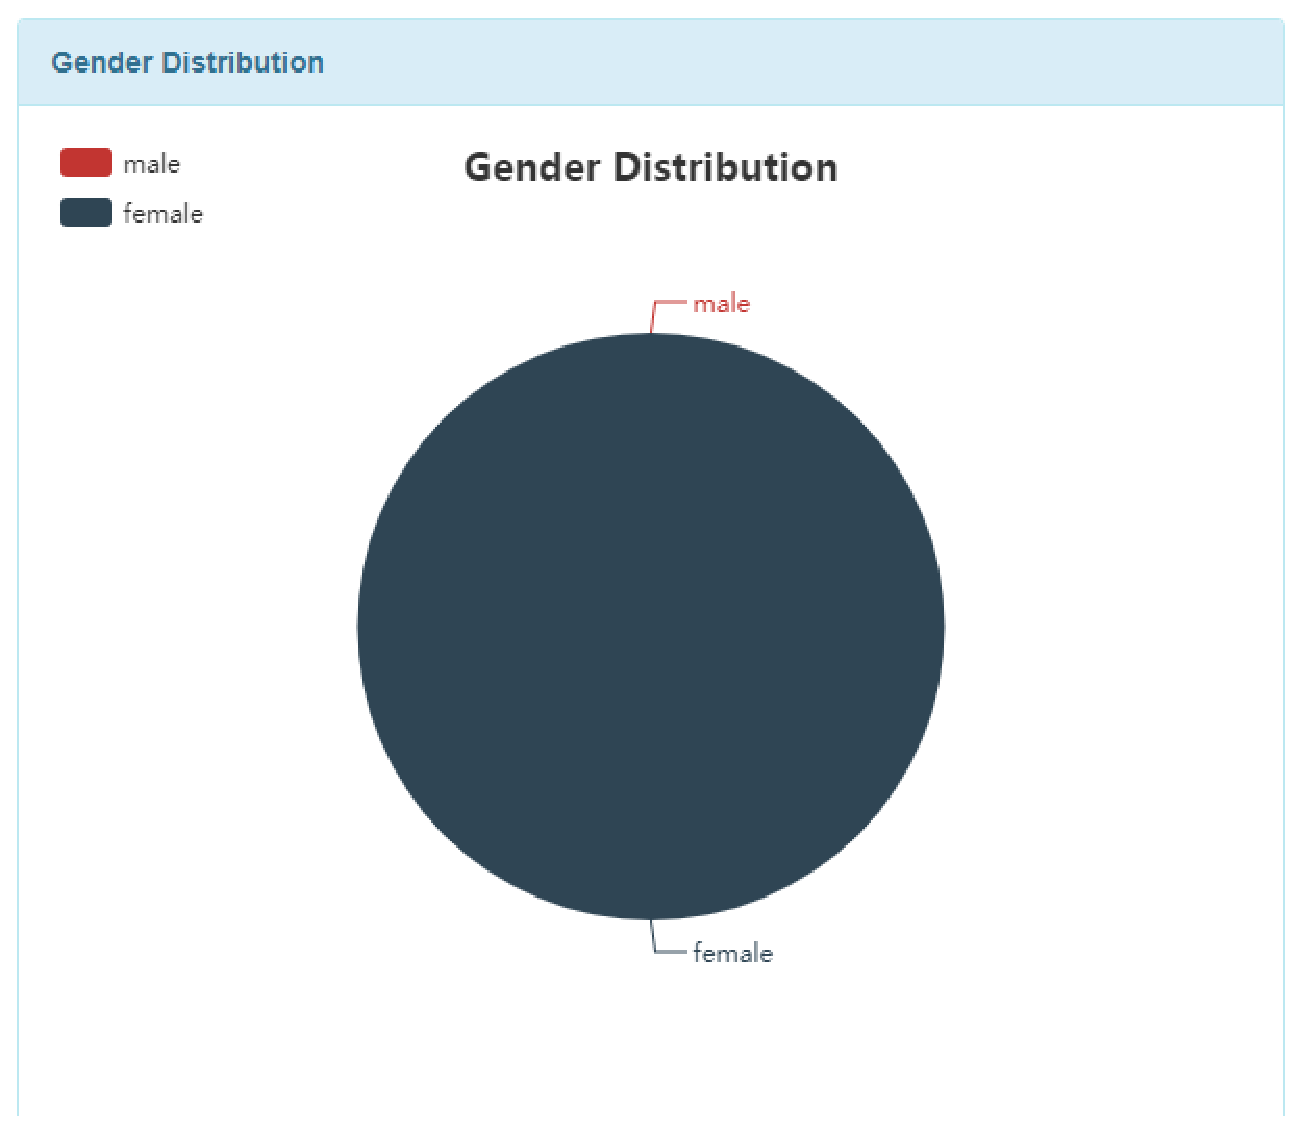
\includegraphics[width=0.23\textwidth]{IMAGE/group-images/21.eps}}
  \subfigure{
  \label{fig:subfig2:fig22}
      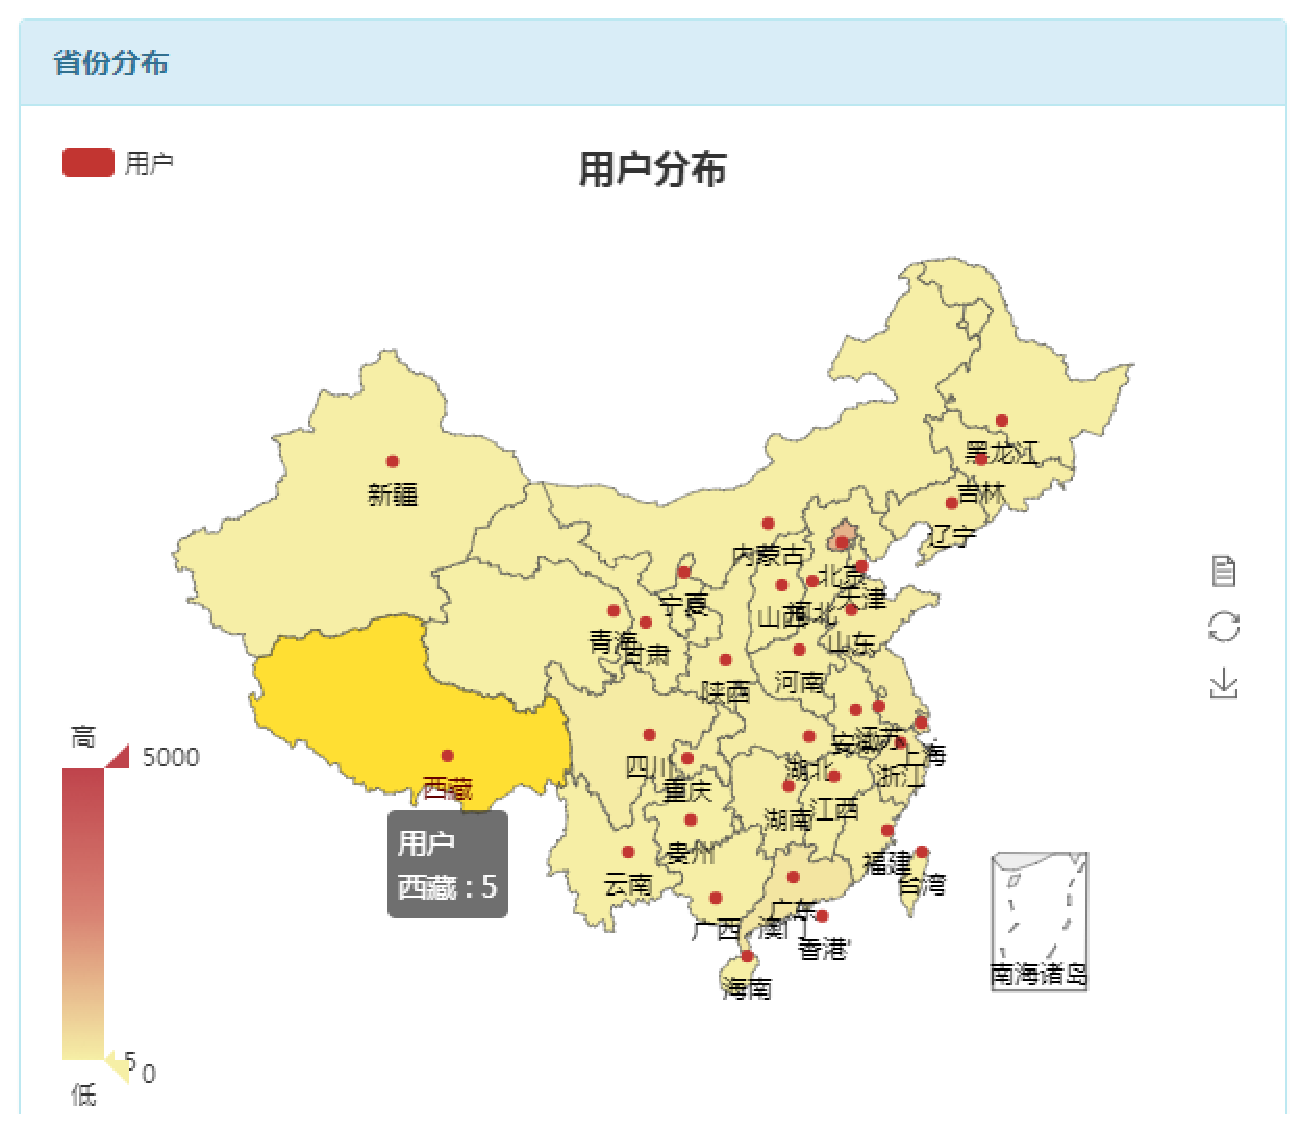
\includegraphics[width=0.23\textwidth]{IMAGE/group-images/22.eps}}
  \subfigure{
  \label{fig:subfig2:fig23}
      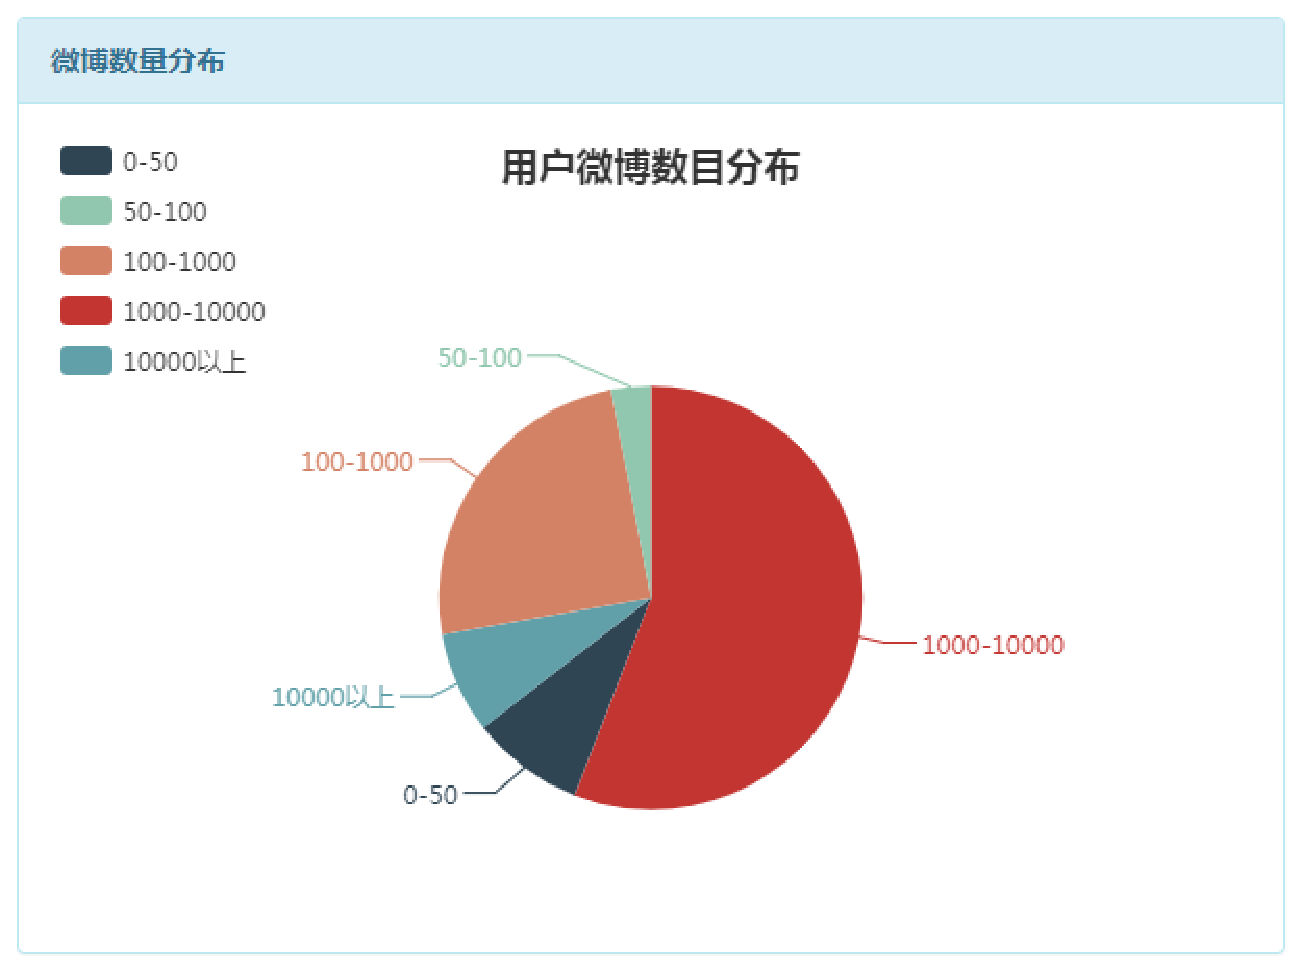
\includegraphics[width=0.23\textwidth]{IMAGE/group-images/23.eps}}
  \subfigure{
  \label{fig:subfig2:fig24}
      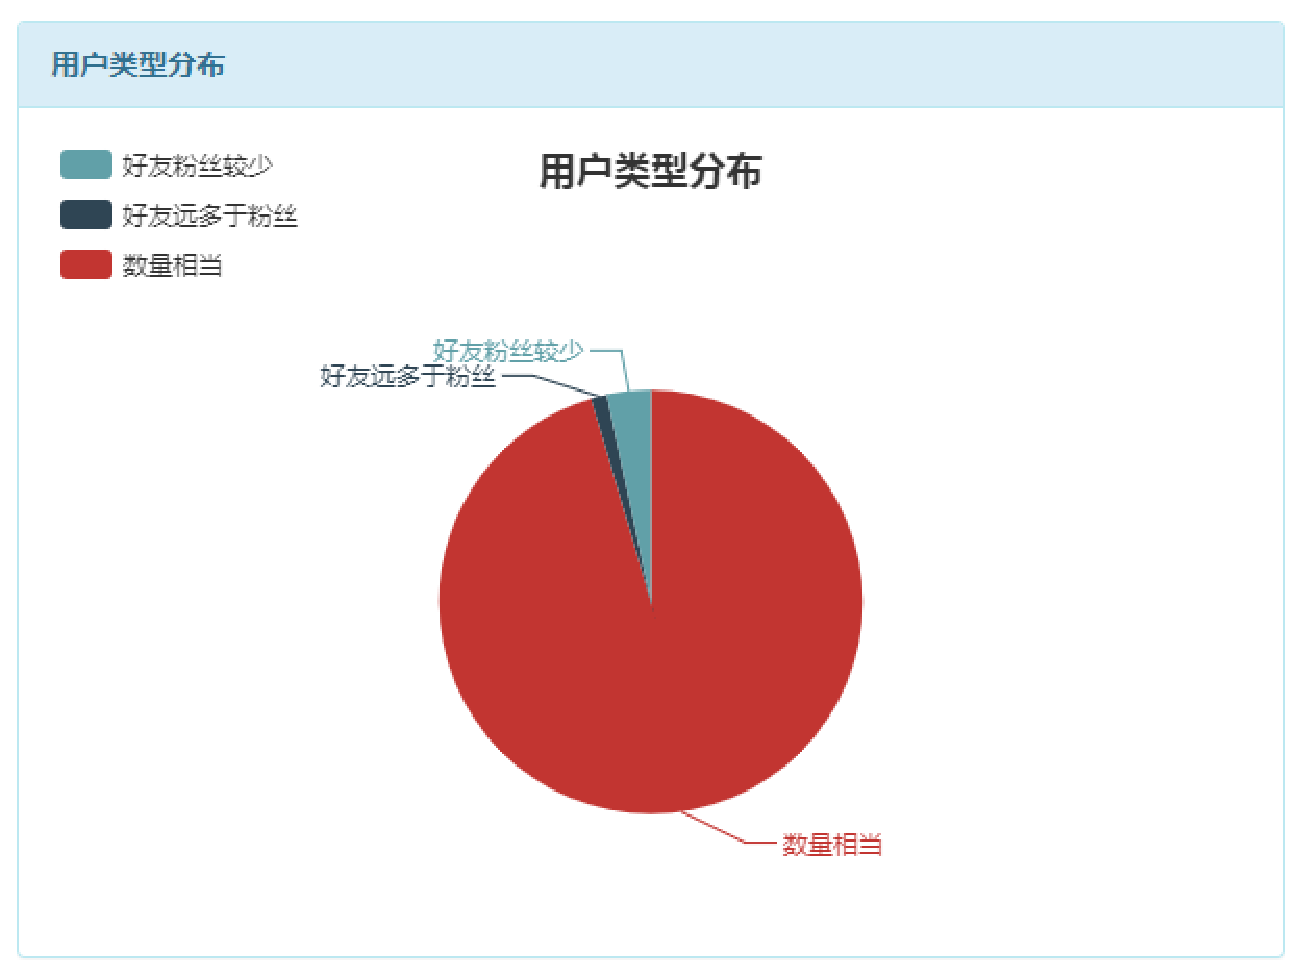
\includegraphics[width=0.23\textwidth]{IMAGE/group-images/24.eps}}
  \subfigure{
  \label{fig:subfig2:fig25}
      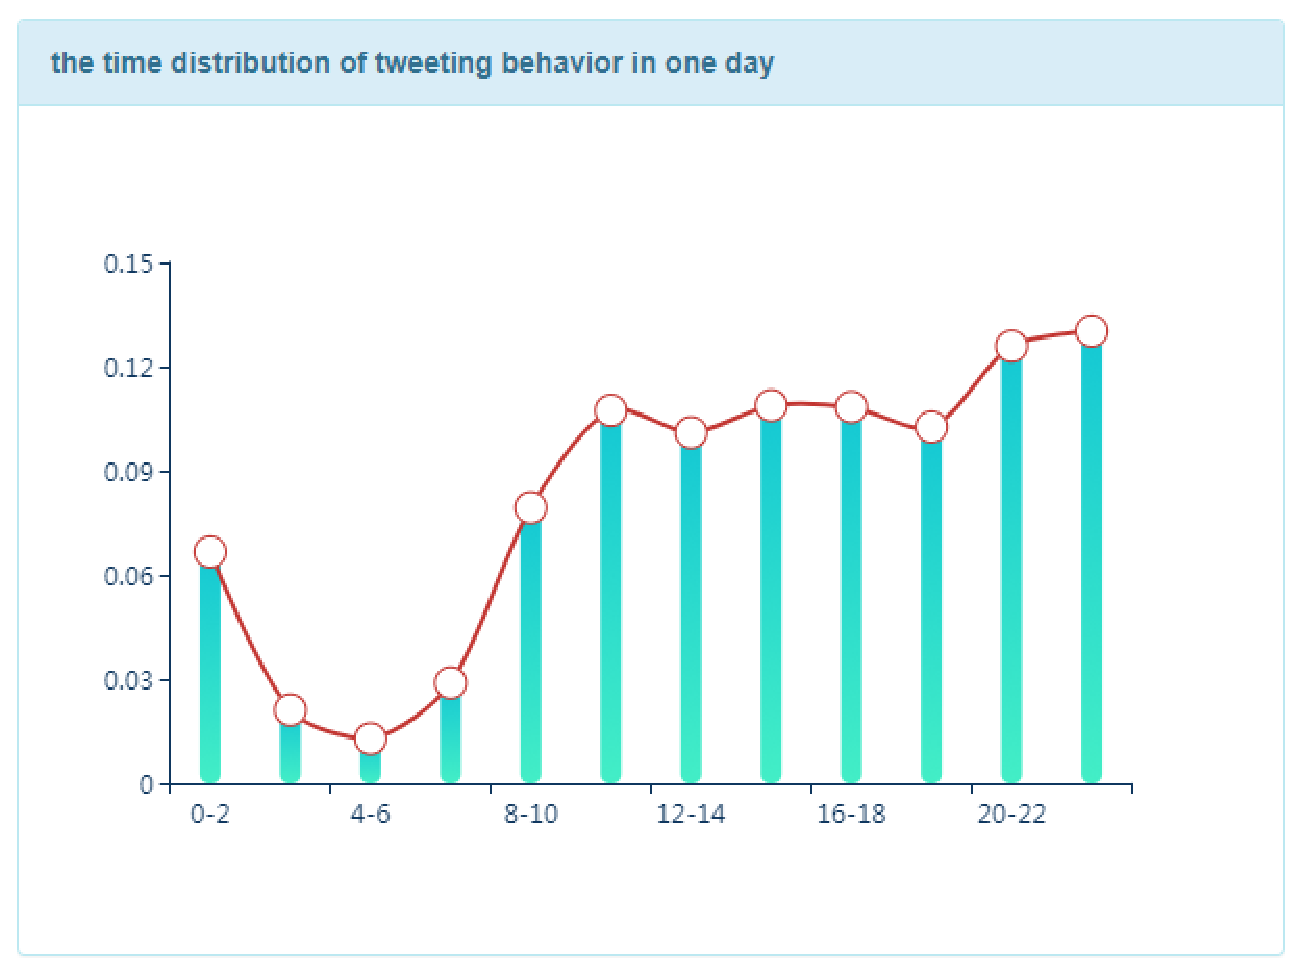
\includegraphics[width=0.23\textwidth]{IMAGE/group-images/25.eps}}
  \subfigure{
  \label{fig:subfig2:fig26}
      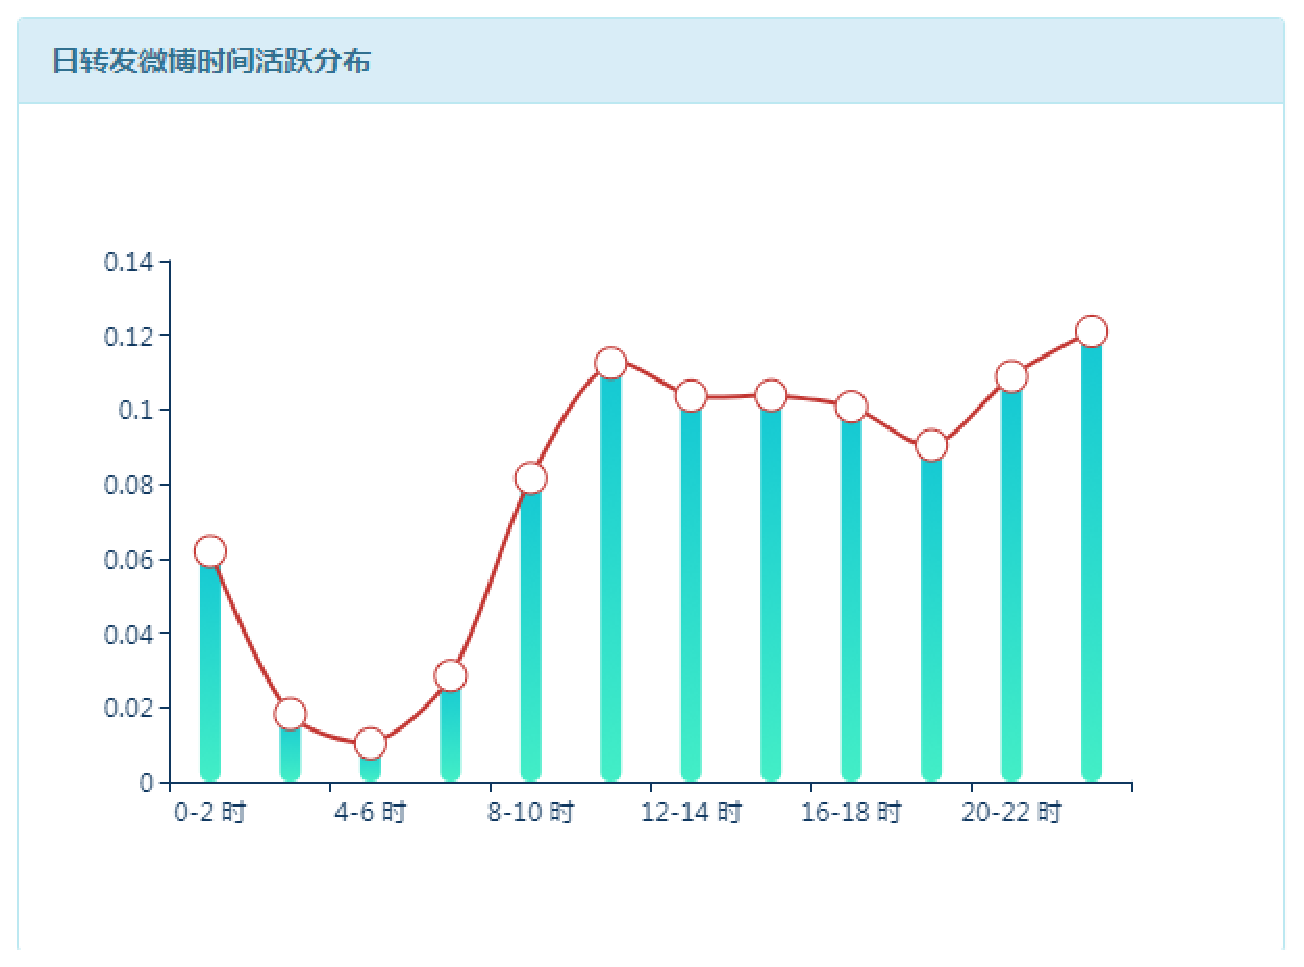
\includegraphics[width=0.23\textwidth]{IMAGE/group-images/26.eps}}
  \subfigure{
  \label{fig:subfig2:fig27}
      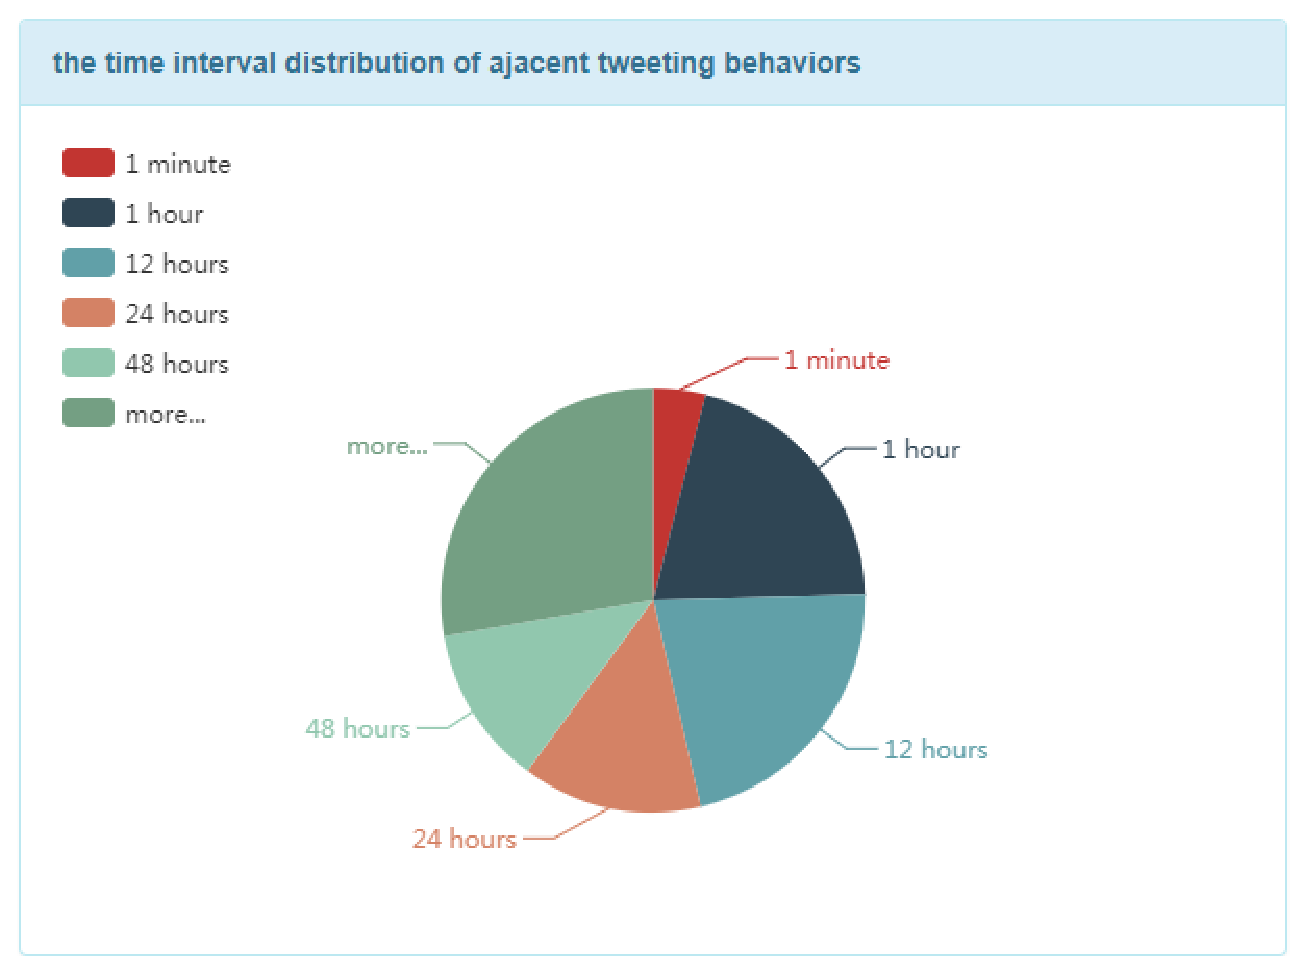
\includegraphics[width=0.23\textwidth]{IMAGE/group-images/27.eps}}
  \subfigure{
  \label{fig:subfig2:fig28}
      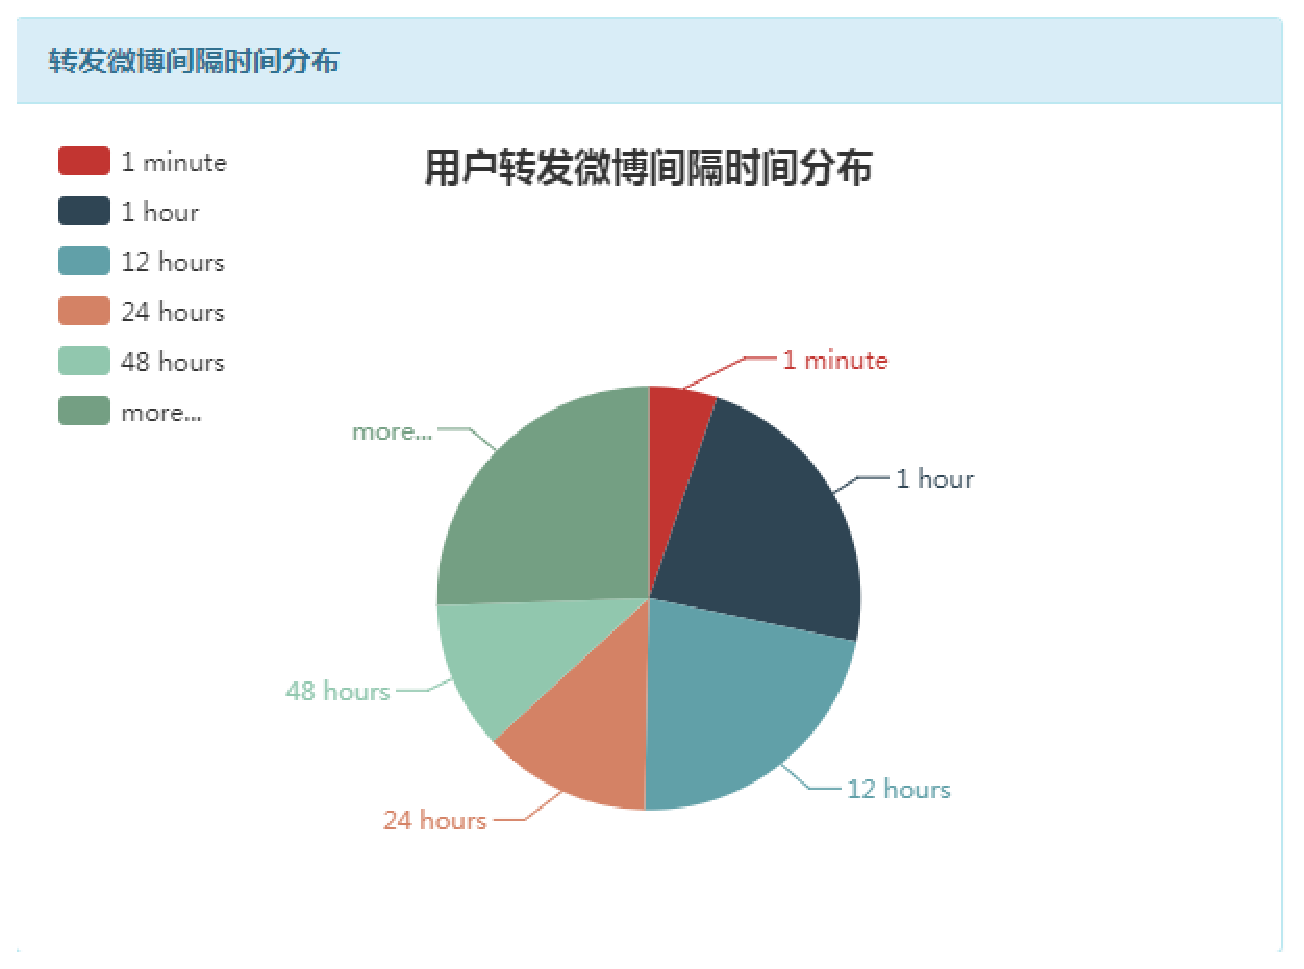
\includegraphics[width=0.23\textwidth]{IMAGE/group-images/28.eps}}
  \subfigure{
  \label{fig:subfig2:fig29}
      
\includegraphics[width=0.23\textwidth]{IMAGE/group-images/29.eps}}
  \caption{The Statistics of User Group Two}
  \label{fig:subfig2} %% label for entire figure
\end{figure*}

\begin{figure*}
  \centering
  \subfigure{
  \label{fig:subfig3:fig31}
      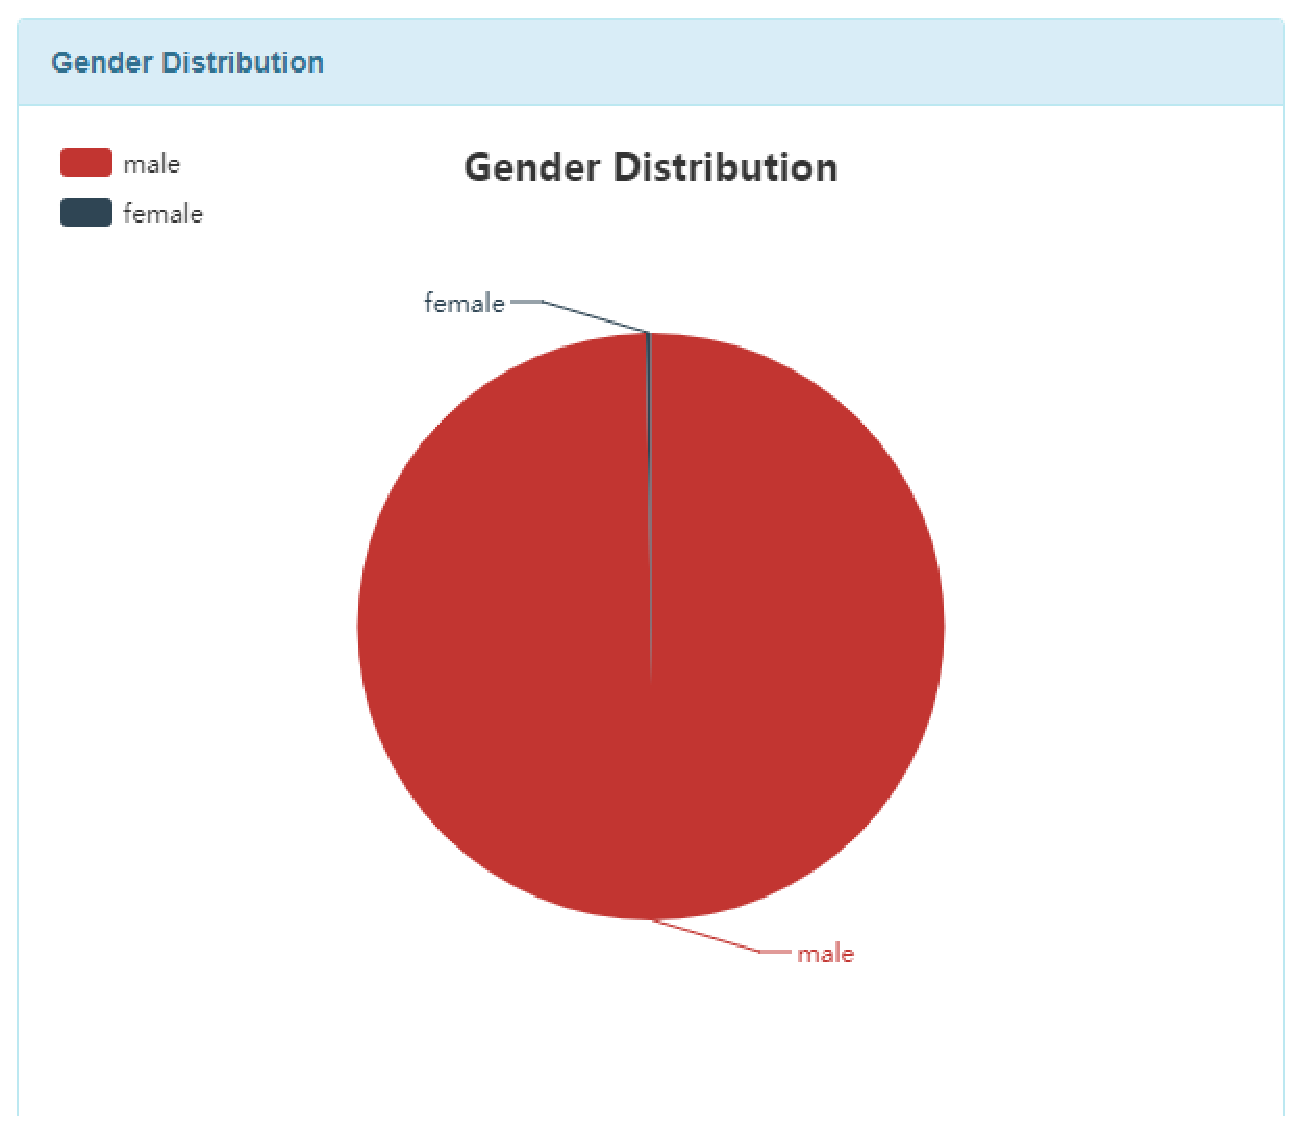
\includegraphics[width=0.23\textwidth]{IMAGE/group-images/31.eps}}
  \subfigure{
  \label{fig:subfig3:fig32}
      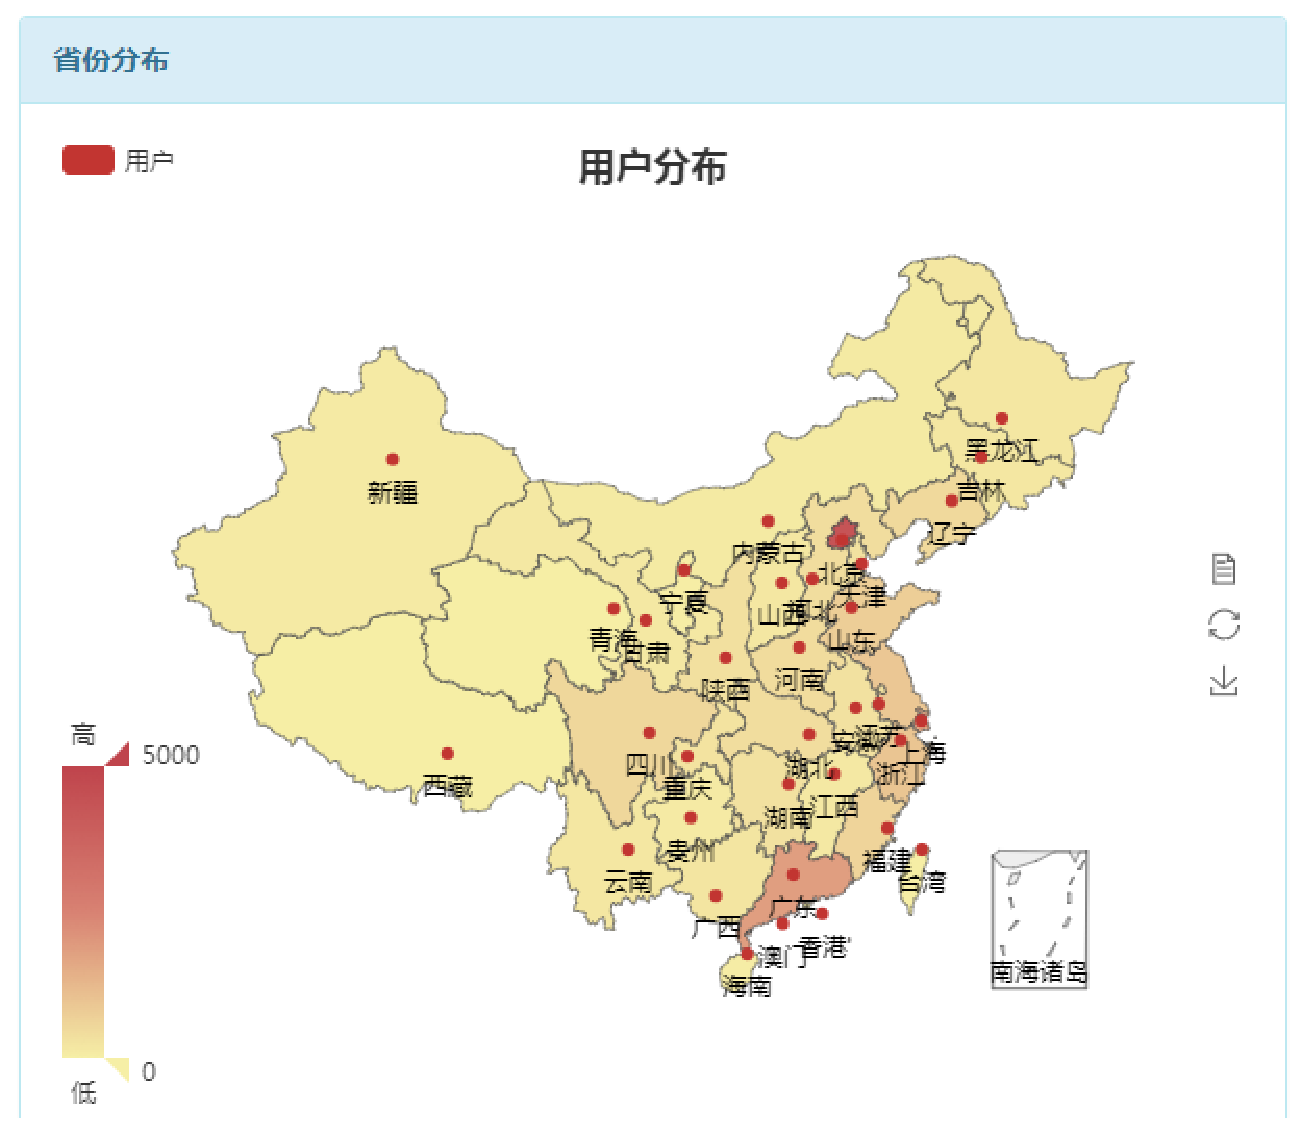
\includegraphics[width=0.23\textwidth]{IMAGE/group-images/32.eps}}
  \subfigure{
  \label{fig:subfig3:fig33}
      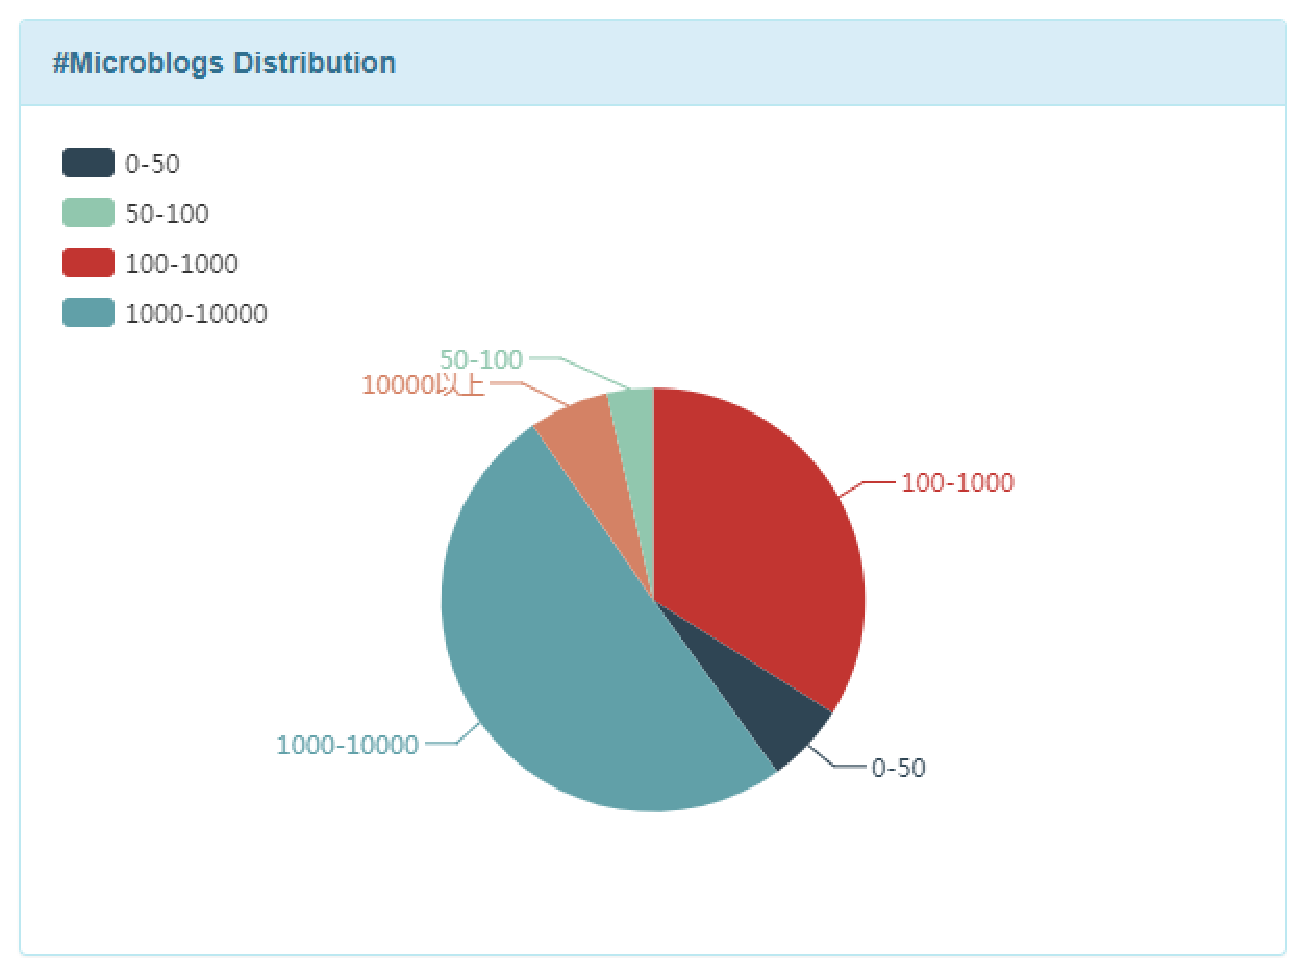
\includegraphics[width=0.23\textwidth]{IMAGE/group-images/33.eps}}
  \subfigure{
  \label{fig:subfig3:fig34}
      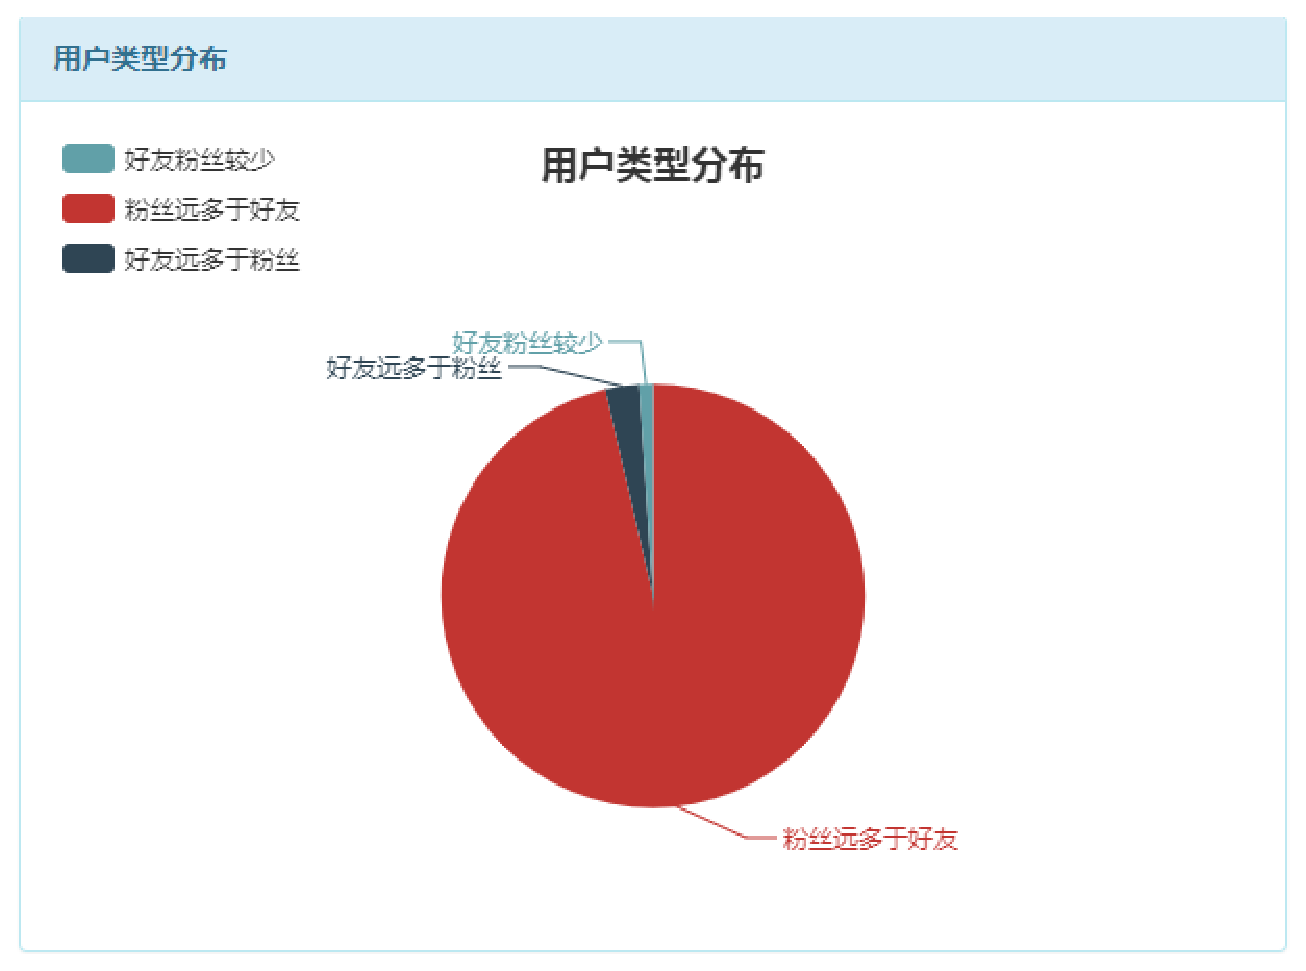
\includegraphics[width=0.23\textwidth]{IMAGE/group-images/34.eps}}
  \subfigure{
  \label{fig:subfig3:fig35}
      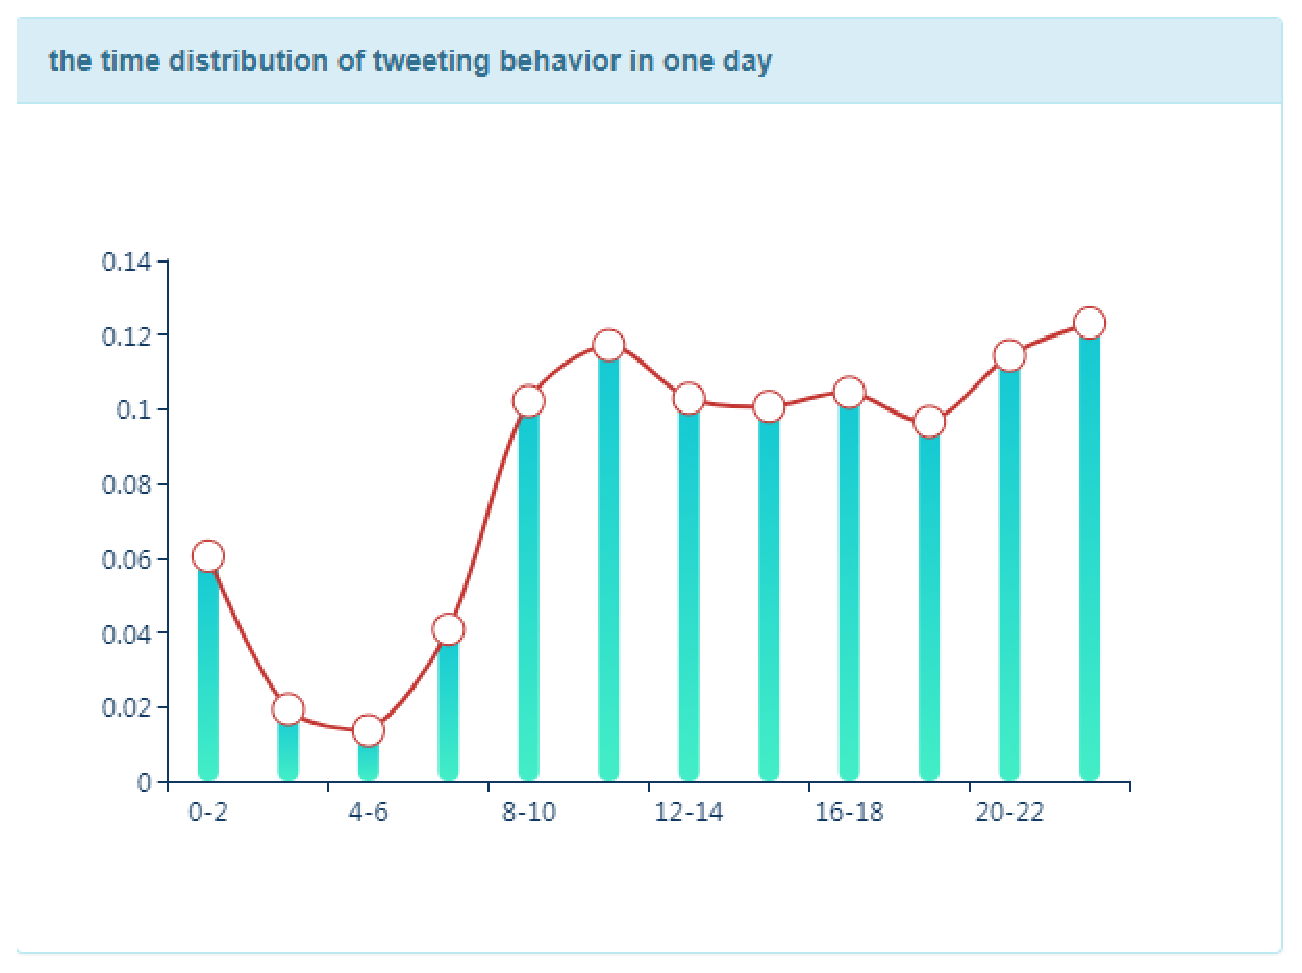
\includegraphics[width=0.23\textwidth]{IMAGE/group-images/35.eps}}
  \subfigure{
  \label{fig:subfig3:fig36}
      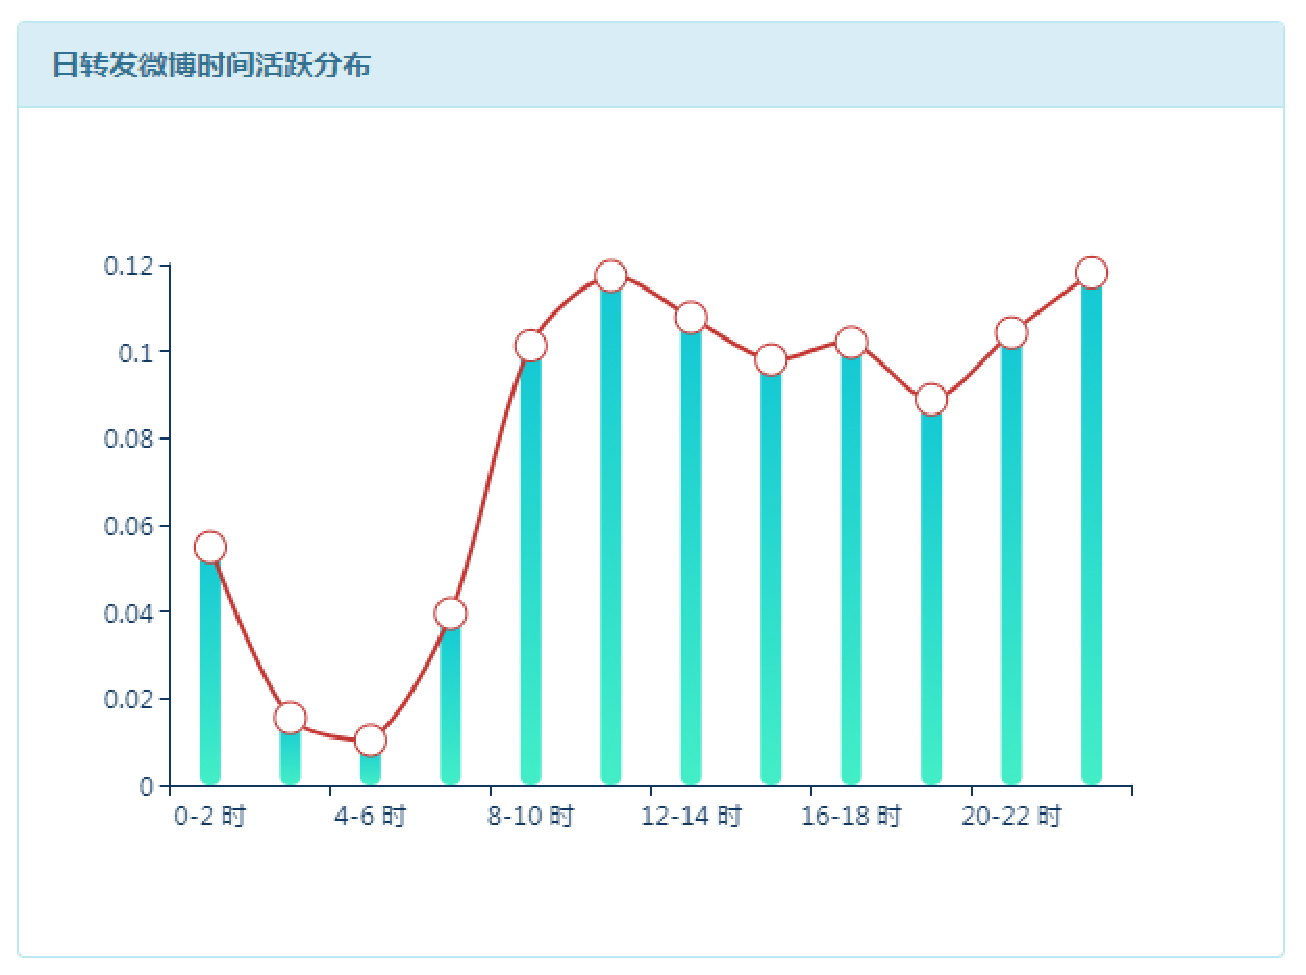
\includegraphics[width=0.23\textwidth]{IMAGE/group-images/36.eps}}
  \subfigure{
  \label{fig:subfig3:fig37}
      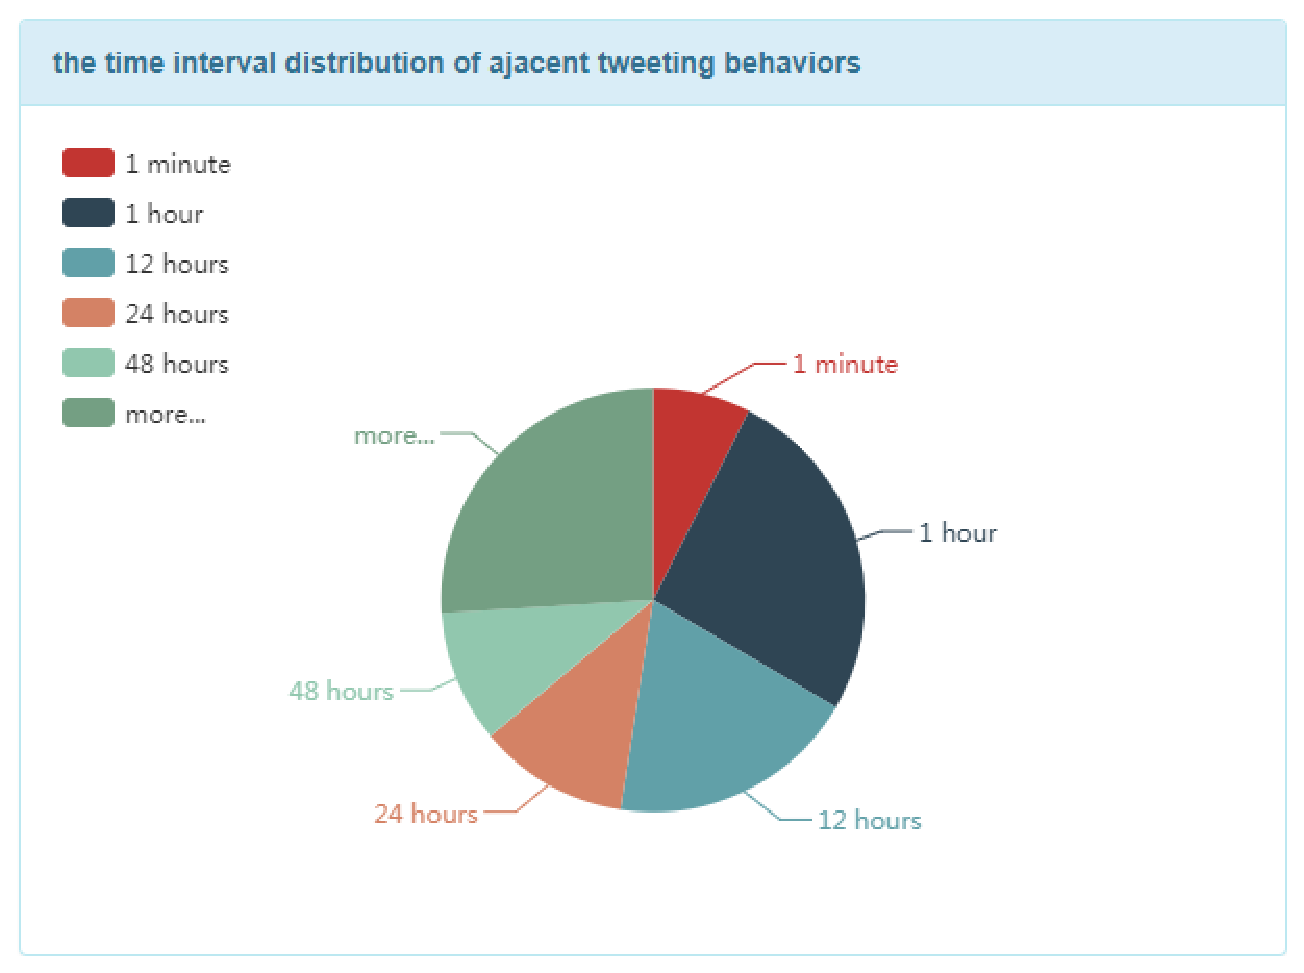
\includegraphics[width=0.23\textwidth]{IMAGE/group-images/37.eps}}
  \subfigure{
  \label{fig:subfig3:fig38}
      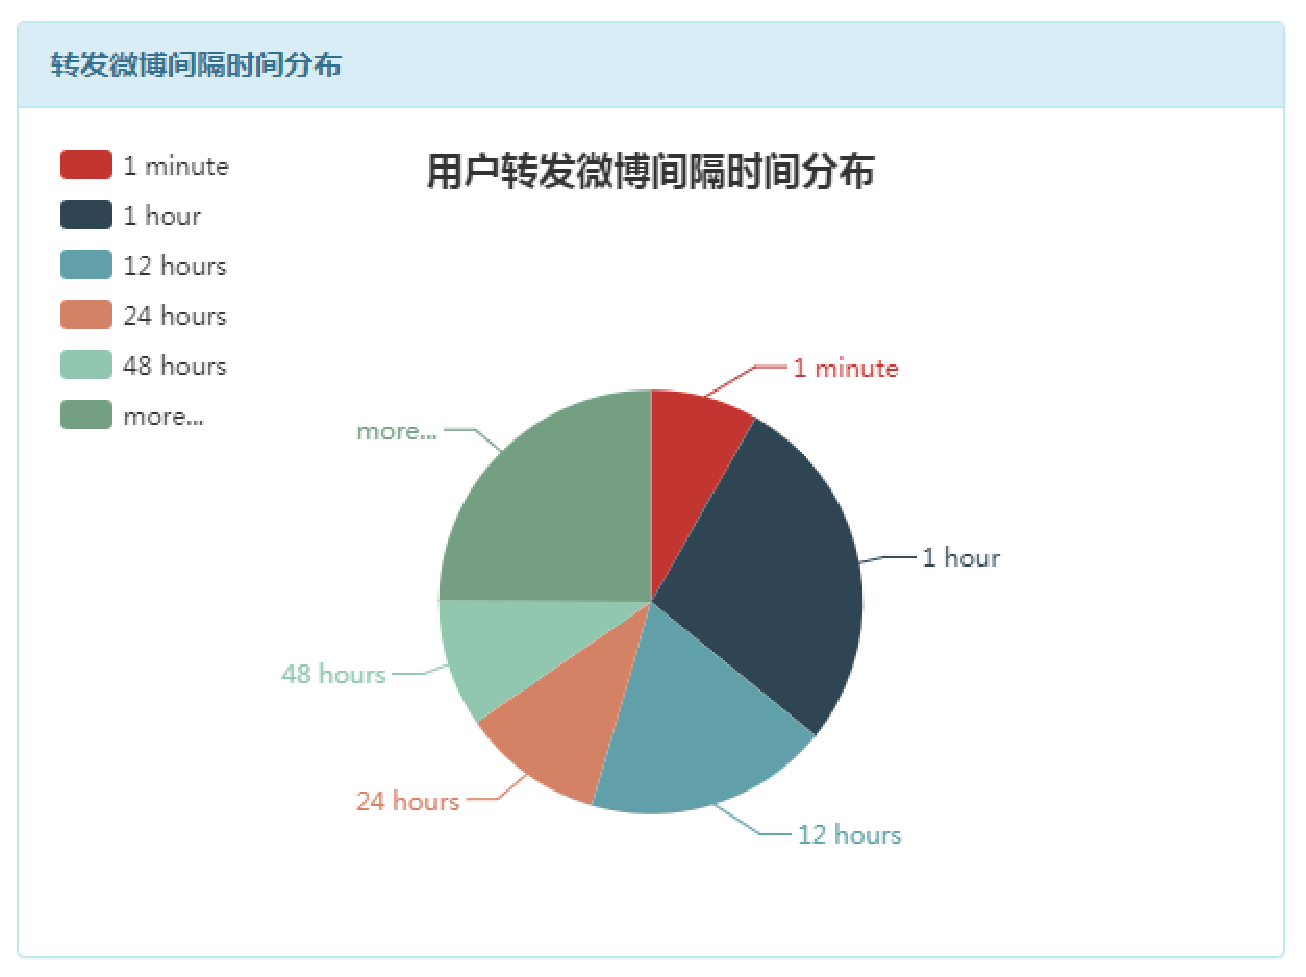
\includegraphics[width=0.23\textwidth]{IMAGE/group-images/38.eps}}
  \subfigure{
  \label{fig:subfig3:fig39}
      
\includegraphics[width=0.23\textwidth]{IMAGE/group-images/39.eps}}
  \caption{The Statistics of User Group Three}
  \label{fig:subfig3} %% label for entire figure
\end{figure*}


\begin{figure*}
  \centering
  \subfigure{
  \label{fig:subfig4:fig41}
      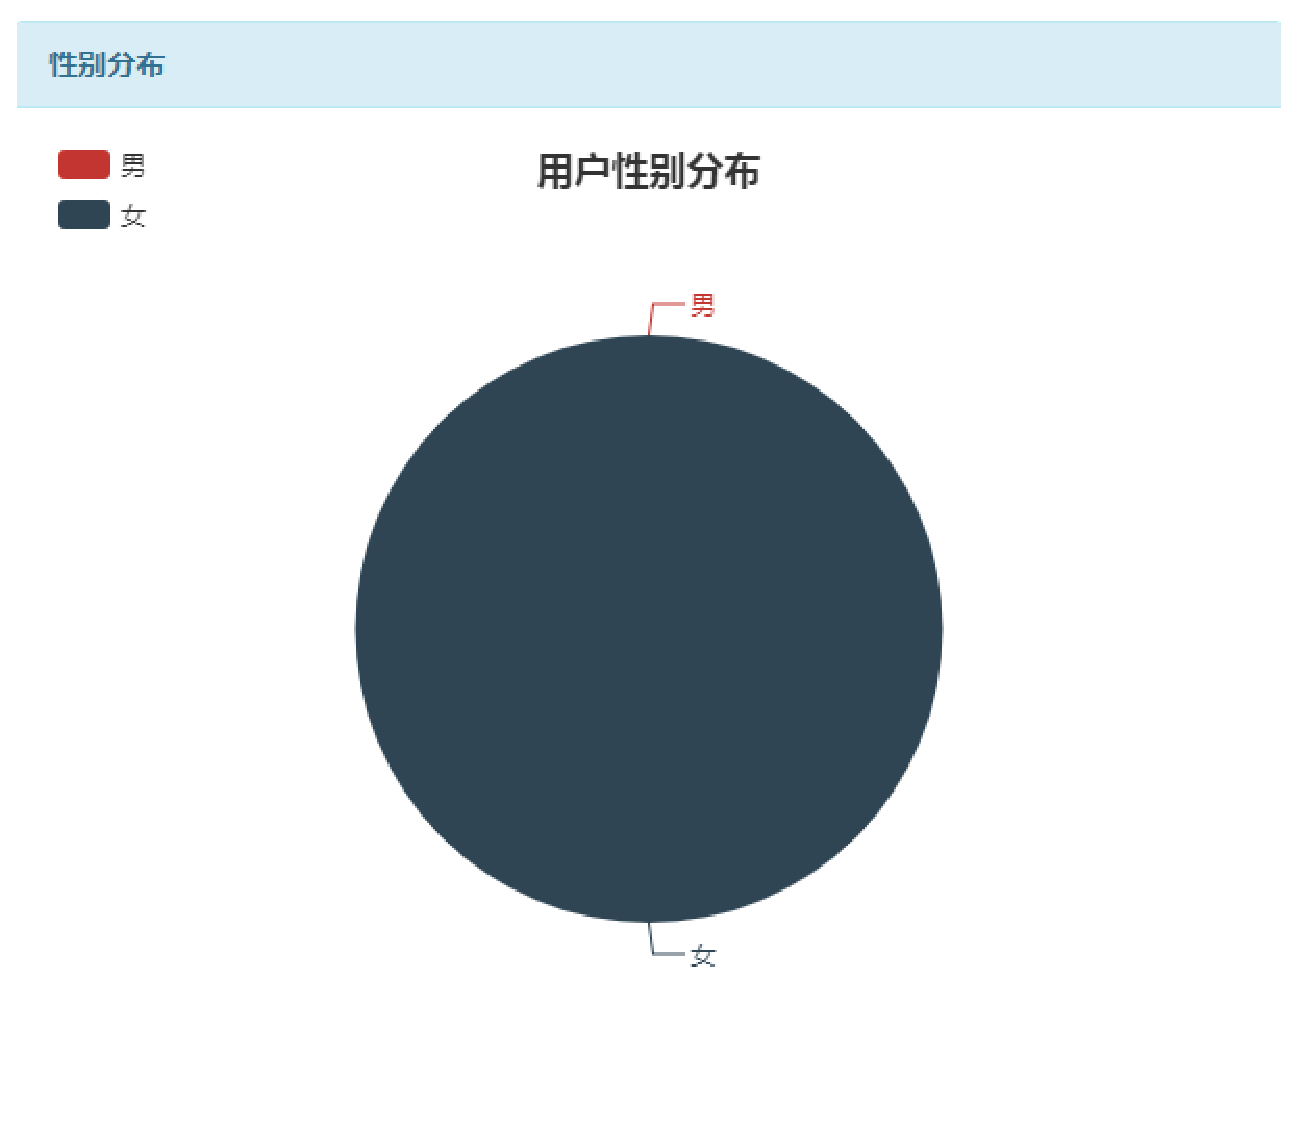
\includegraphics[width=0.23\textwidth]{IMAGE/group-images/41.eps}}
  \subfigure{
  \label{fig:subfig4:fig42}
      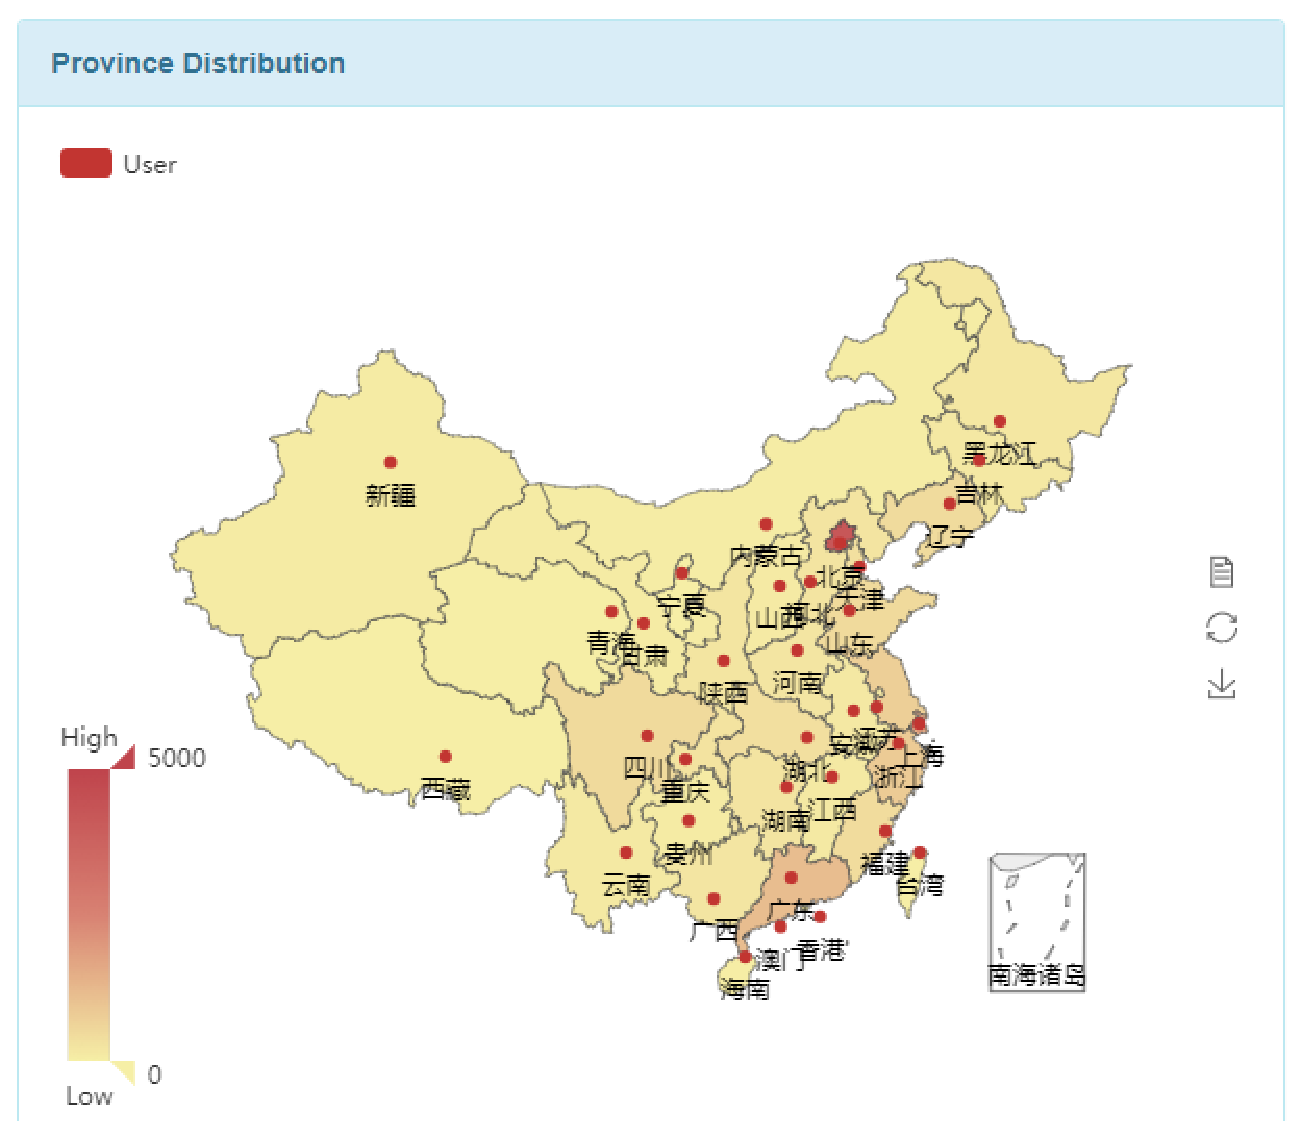
\includegraphics[width=0.23\textwidth]{IMAGE/group-images/42.eps}}
  \subfigure{
  \label{fig:subfig4:fig43}
      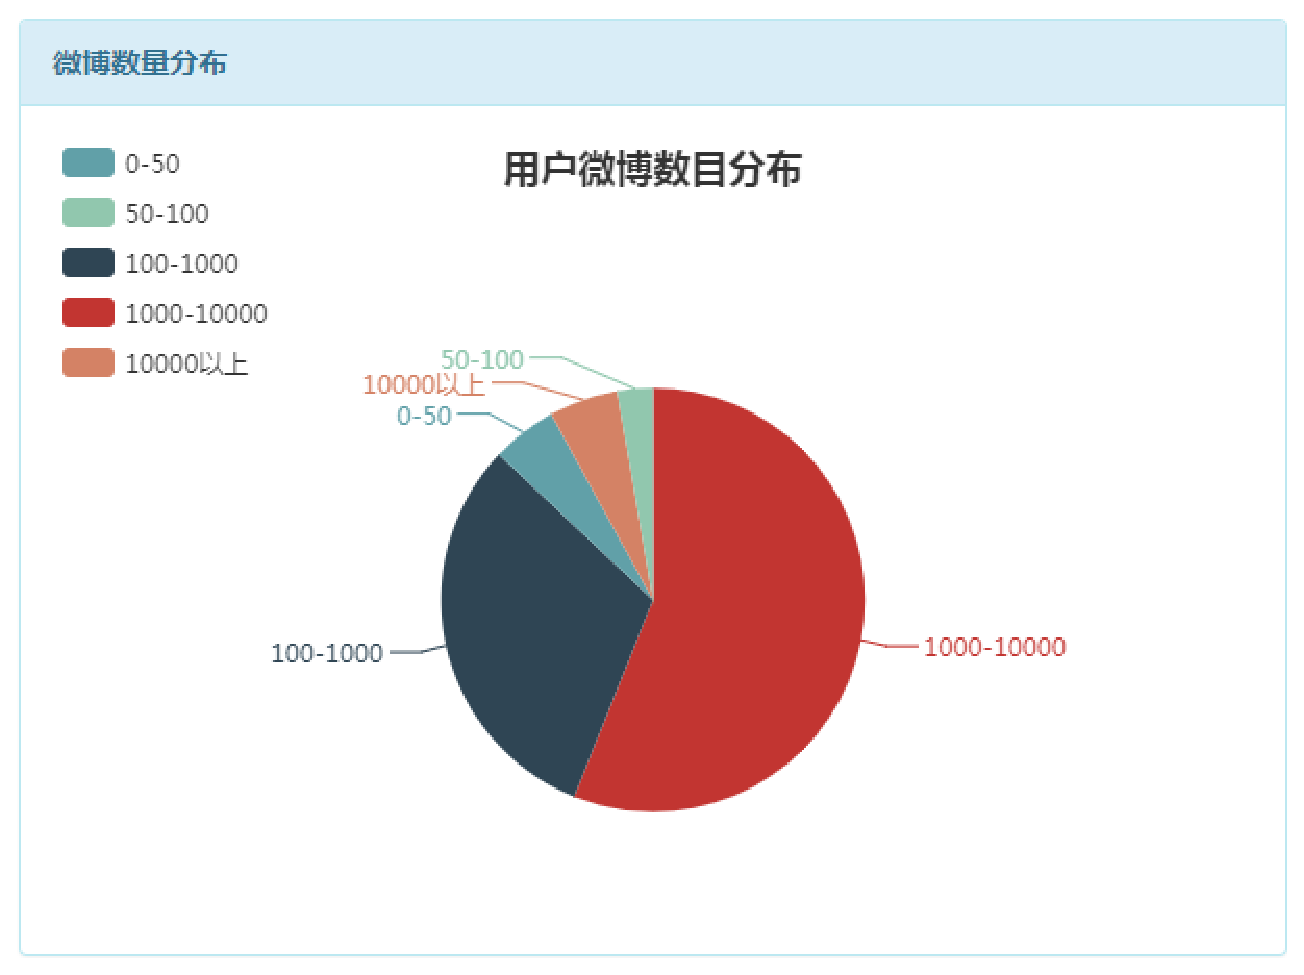
\includegraphics[width=0.23\textwidth]{IMAGE/group-images/43.eps}}
  \subfigure{
  \label{fig:subfig4:fig44}
      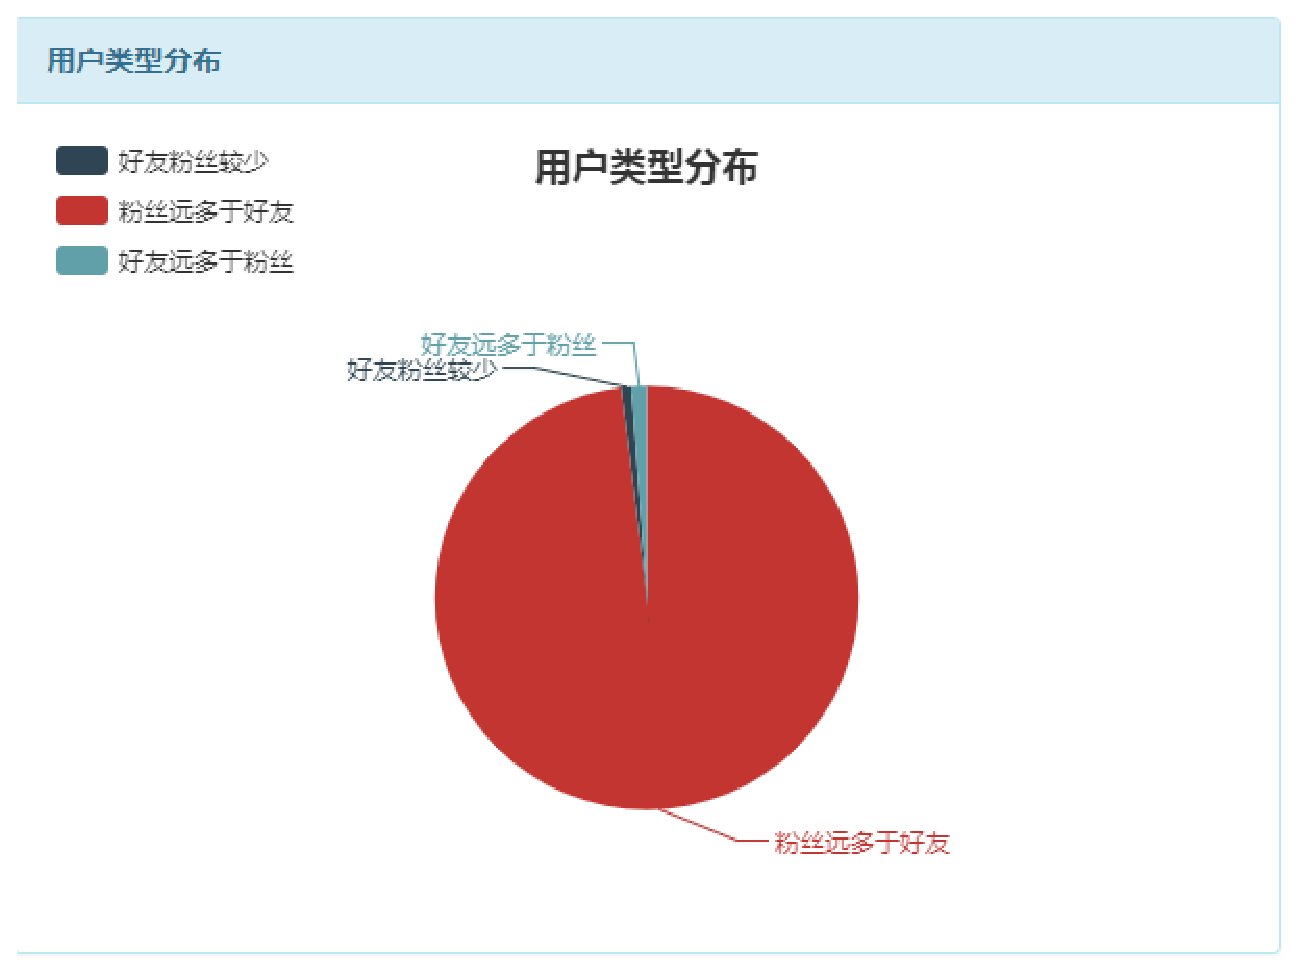
\includegraphics[width=0.23\textwidth]{IMAGE/group-images/44.eps}}
  \subfigure{
  \label{fig:subfig4:fig45}
      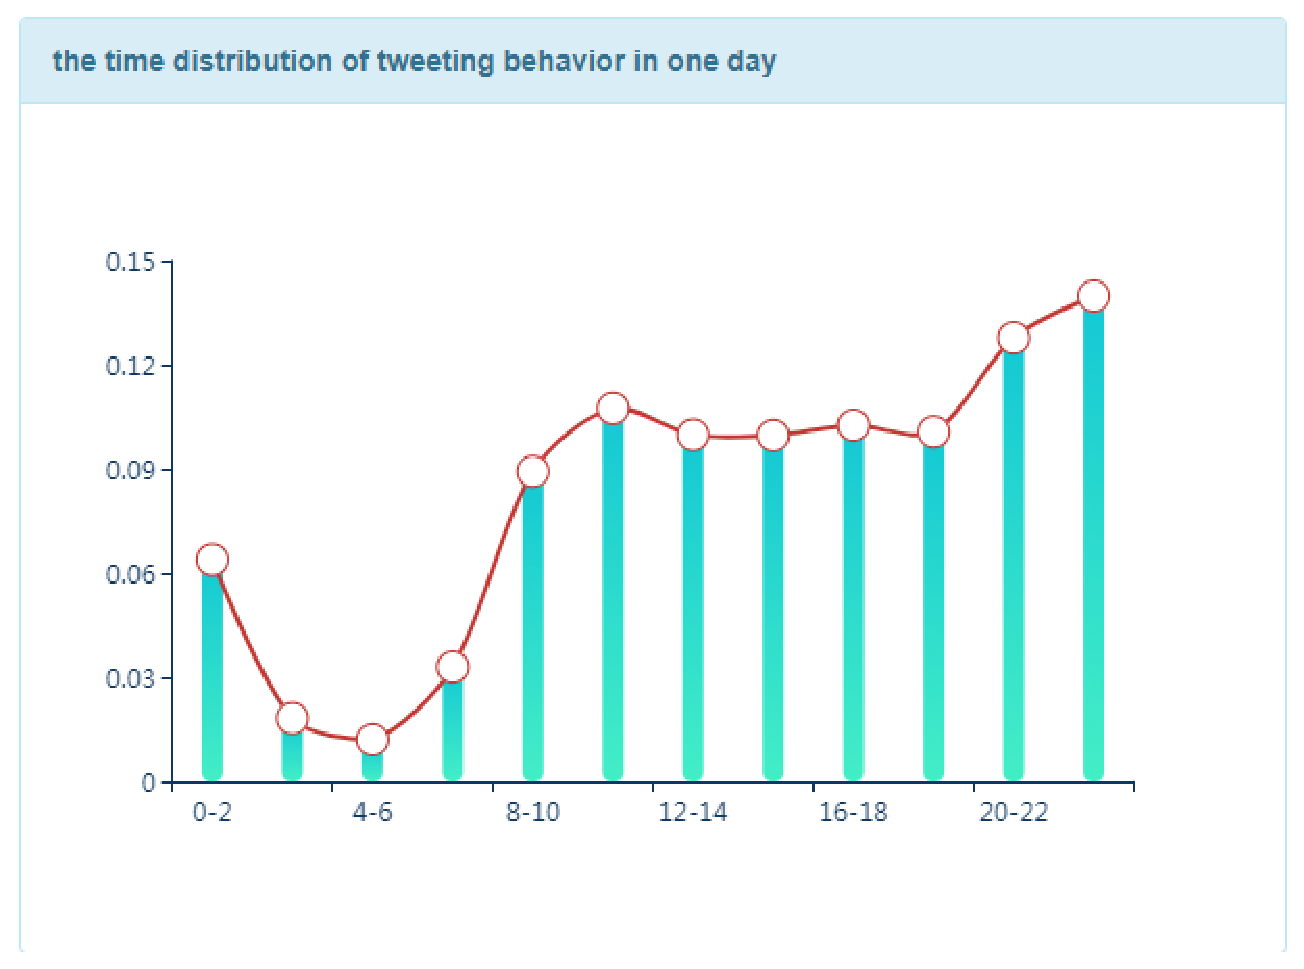
\includegraphics[width=0.23\textwidth]{IMAGE/group-images/45.eps}}
  \subfigure{
  \label{fig:subfig4:fig46}
      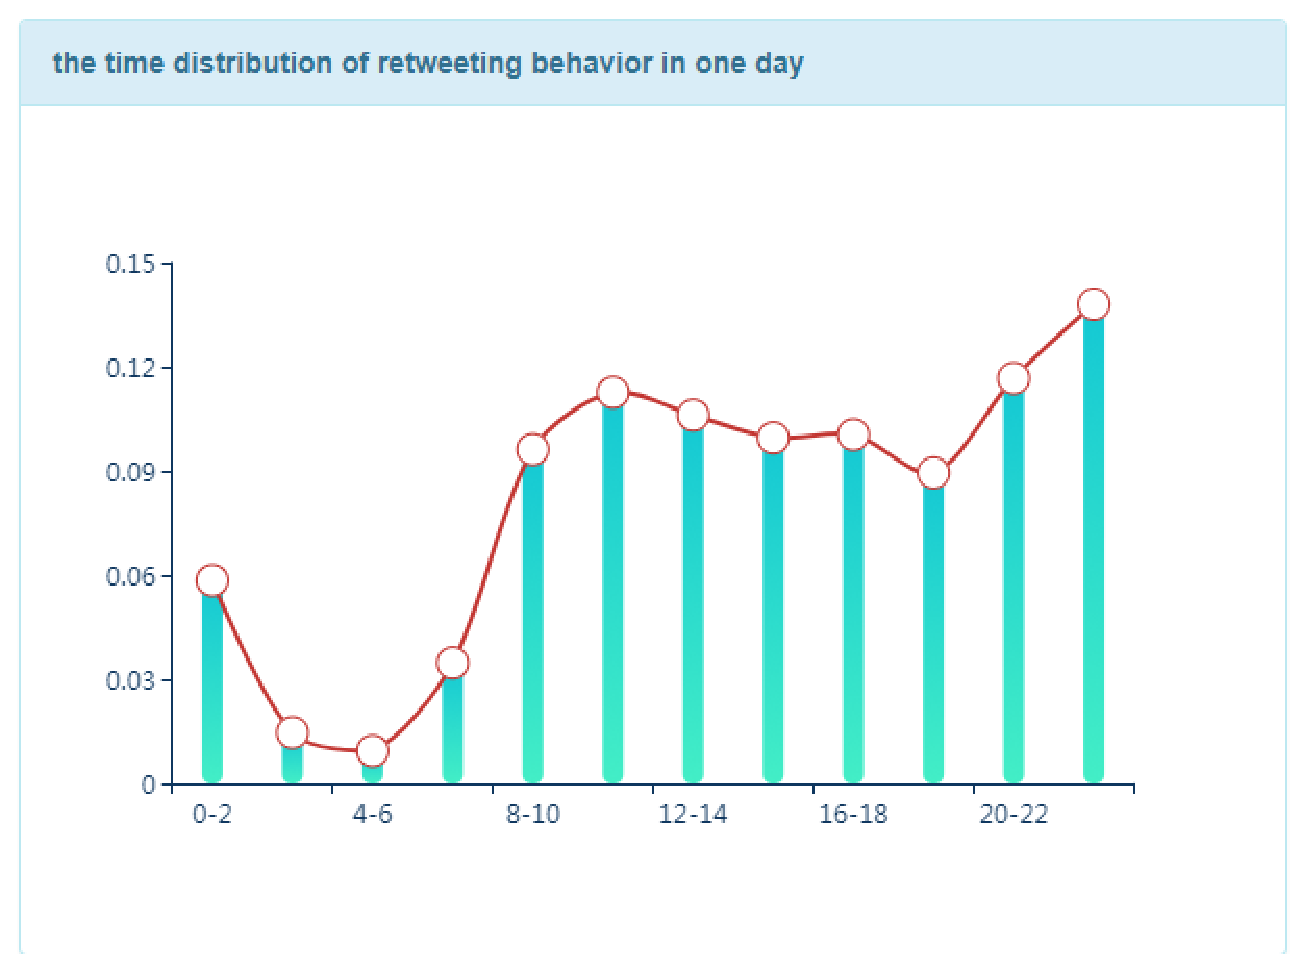
\includegraphics[width=0.23\textwidth]{IMAGE/group-images/46.eps}}
  \subfigure{
  \label{fig:subfig4:fig47}
      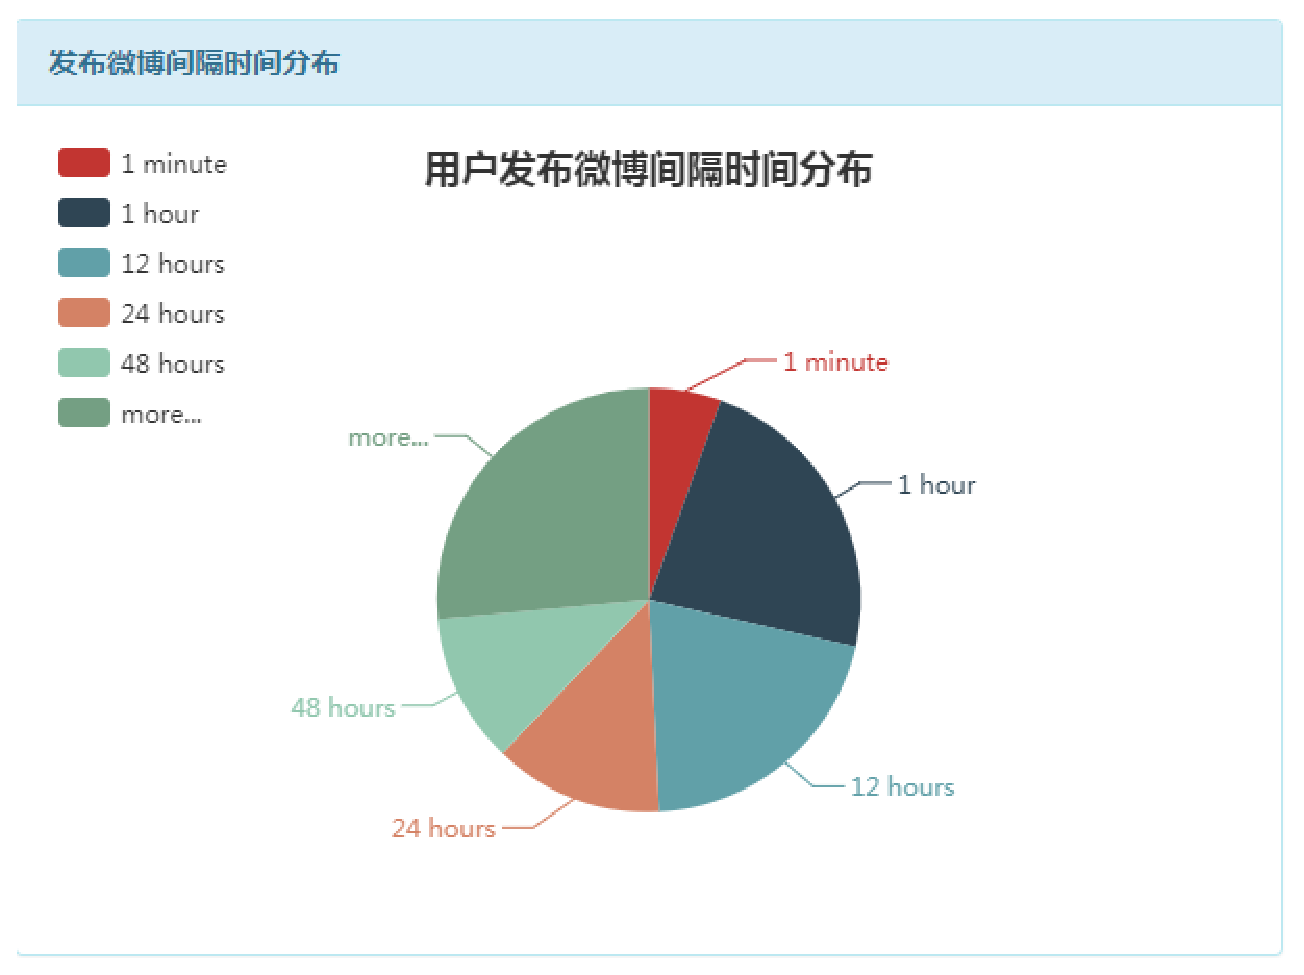
\includegraphics[width=0.23\textwidth]{IMAGE/group-images/47.eps}}
  \subfigure{
  \label{fig:subfig4:fig48}
      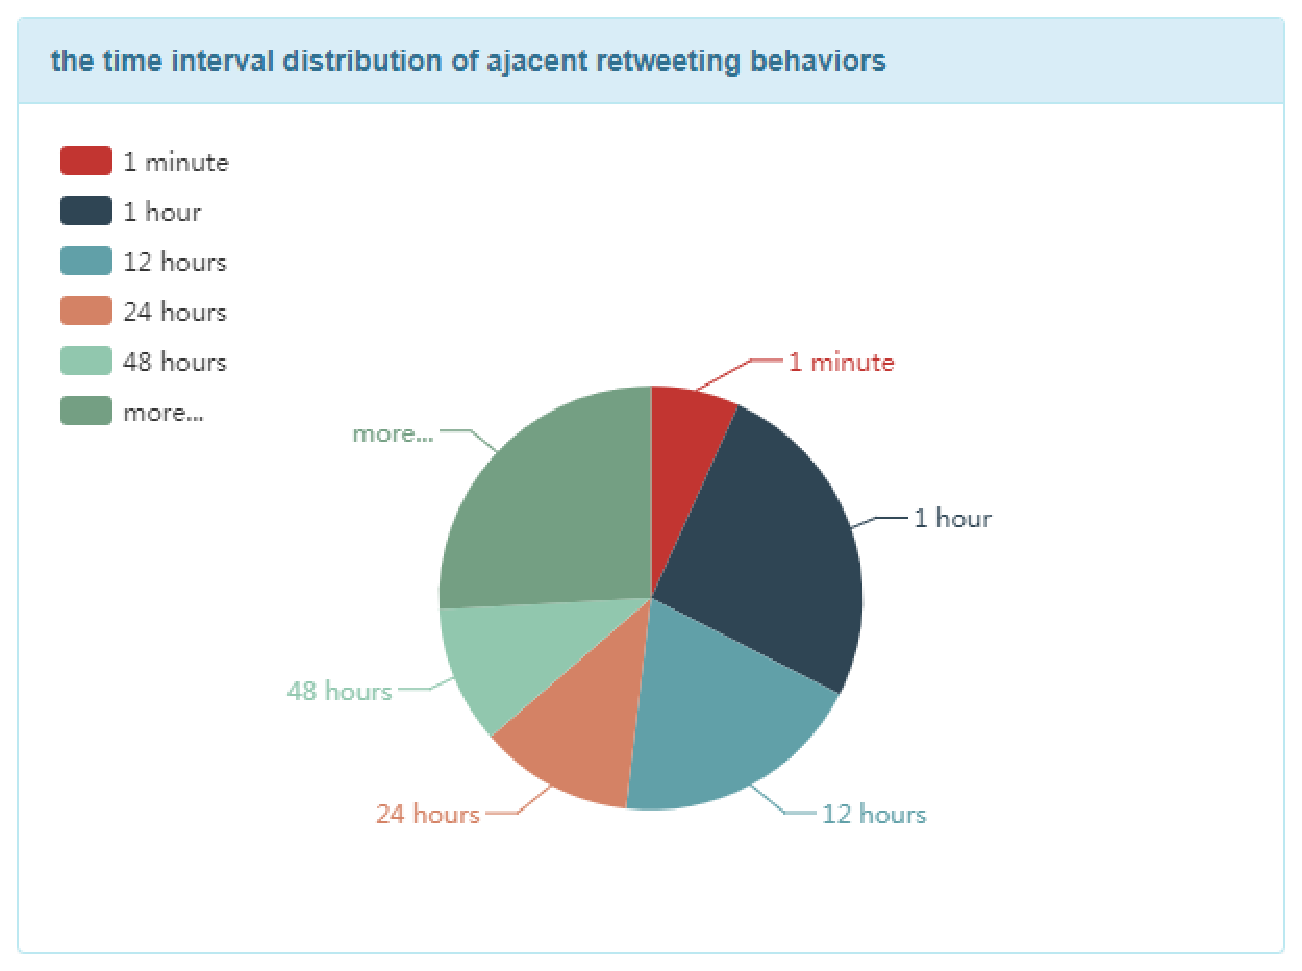
\includegraphics[width=0.23\textwidth]{IMAGE/group-images/48.eps}}
  \subfigure{
  \label{fig:subfig4:fig49}
      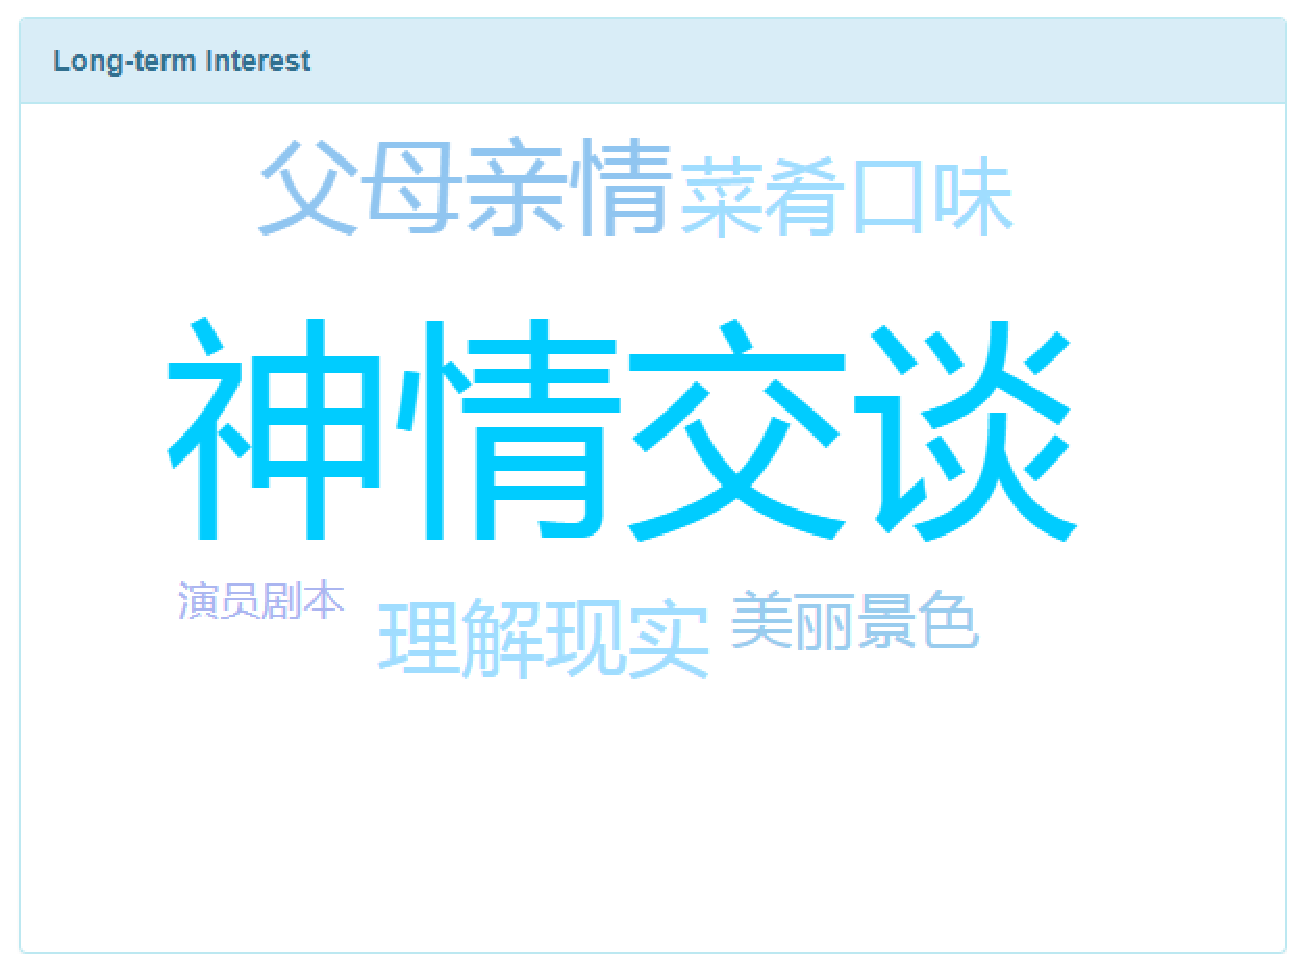
\includegraphics[width=0.23\textwidth]{IMAGE/group-images/49.eps}}
  \caption{The Statistics of User Group Four}
  \label{fig:subfig4} %% label for entire figure
\end{figure*}
